\documentclass[conference]{IEEEtran}

\usepackage{pythonhighlight}
\documentclass{article}
\usepackage{graphicx}
\usepackage{subcaption} 
\usepackage{graphicx}
\usepackage{hyperref}
\usepackage{float}
\usepackage[english]{babel}
\usepackage{listings} % code blocks
\usepackage[utf8]{inputenc}
\usepackage{amsmath}
\usepackage[acronym]{glossaries}
\makeglossaries
%\usepackage{etoolbox} % citações

\hyphenation{}

\begin{document}
% paper title
% can use linebreaks \\ within to get better formatting as desired
\title{Intel Image Scene Classification of Landscapes}

% author names and affiliations
% use a multiple column layout for up to three different
% affiliations
\author{
    \IEEEauthorblockN{Nelson Loureiro}
   \IEEEauthorblockA{
        Fundamentos de Aprendizagem Automática 24/25\\
        Departamento de Eletrónica, Telecomunicações e Informática\\
        University of Aveiro\\
        Aveiro, Portugal\\
        nelson.loureiro@ua.pt
    }
    \and
    \IEEEauthorblockN{Cristiano Nicolau}
    \IEEEauthorblockA{
        Fundamentos de Aprendizagem Automática 24/25\\
        Departamento de Eletrónica, Telecomunicações e Informática\\
        University of Aveiro\\
        Aveiro, Portugal\\
        cristianonicolau@ua.pt
    }
}
% make the title area
\maketitle

\begin{abstract}
This project focuses on image scene classification using the Intel Image Classification dataset, which contains images categorized into six classes: buildings, forest, glacier, mountain, sea, and street. We implemented convolutional neural networks (CNNs), including DenseNet and a Forward Neural Network, to develop models capable of accurately classifying these scenes. The models were further enhanced using data augmentation techniques and hyperparameter tuning to optimize performance. This work has implications for applications in geospatial analysis, urban planning, and environmental monitoring.
\end{abstract}

\begin{center}
    \textit{\textbf{Keywords} —Intel Image Classification, Image Scene Classification, Machine Learning, Multiclass Classification, Neural Network, Deep Learning, CNN, Convolutional Neural Network}
\end{center}
\IEEEpeerreviewmaketitle
%\acrlong{da}
%\acrshort{da}
%\acrfull{da}

\newacronym{ml}{ML}{Machine Learning}
\newacronym{svm}{SVM}{Support Vector Machine} 
\newacronym{mlp}{MLP}{Multi-layer Perceptrons}
\newacronym{fnn}{FNN}{Feedforward Neural Network}
\newacronym{TP}{TP}{True Positive}
\newacronym{FP}{FP}{False Positive}
\newacronym{TN}{TN}{True Negative}
\newacronym{FN}{FN}{False Negative}

\section{Introduction}
\label{sec:Introduction}
Scene image classification is an increasingly vital domain within computer vision, underpinning a wide range of applications such as medical diagnostics, autonomous navigation, environmental monitoring, digital content recommendation, and tourism planning. Unlike basic image classification, which typically focuses on identifying individual objects within an image, scene classification involves analyzing complex and diverse visual environments, making it a more challenging yet impactful task.

This paper aims at two key objectives. First, it provides a comprehensive review of the latest advances in scene image classification, critically analyzing, and comparing other studies in the field. Second, it develops, optimizes, and evaluates distinct Feed-Forward Neural Networks (FNNs), and Convolutional Neural Network (CNN) architectures using the Intel Image Classification dataset. This dataset comprises a diverse collection of natural scene images from various global locations, posing a challenging multi-class classification problem.

Our study highlights the effectiveness of different machine learning approaches in accurately classifying images into categories such as buildings, forests, glaciers, mountains, seas, and streets. The paper concludes with a detailed comparative analysis of the model performance and offers key insights derived from the experiments, contributing to the ongoing development of robust and scalable scene classification systems.

\section{State of the Art} \label{sec}

A comprehensive state-of-the-art review was performed to find the most suitable models for application to this dataset and identify the types of studies that had already been conducted.

\subsection{Traditional Machine Learning Approaches}

Before the advent of neural networks, traditional machine learning algorithms dominated image classification tasks. Methods such as Support Vector Machines (SVMs) and Random Forests were widely used. For example, \cite{svm_example} demonstrated the effectiveness of SVMs in high-dimensional spaces, while \cite{rf_example} highlighted the robustness of Random Forests against overfitting in various applications.

Despite their impact, these approaches required manual feature extraction, which was not only labor intensive but also often incapable of capturing intricate patterns in visual data. This limited their ability to handle complex or large-scale datasets, paving the way for deep learning-based solutions.

\subsection{Feedforward Neural Networks (FNNs)}

Feedforward neural networks (FNNs) were among the first models to be applied to image classification problems. Despite their structural simplicity and the ability to solve basic tasks, FNNs lack specific mechanisms to capture the spatial relationships between image pixels, limiting their performance in more complex tasks. However, they served as an important starting point for exploring more sophisticated networks.

\subsection{Convolutional Neural Networks (CNNs)}

The introduction of Convolutional Neural Networks (CNNs) revolutionized the field of image classification by eliminating the need for manual feature extraction. CNNs automatically learn hierarchical representations of images, starting from simple features like edges to complex patterns.

AlexNet \cite{alexnet} was a milestone in this advancement, winning the ImageNet Large Scale Visual Recognition Challenge (ILSVRC) in 2012 and demonstrating the potential of deep networks in visual recognition. Later, VGGNet \cite{vgnet} introduced a deeper architecture with smaller convolutional filters and a consistent structure, becoming a reference for many image classification tasks due to its simplicity and effectiveness.

\subsection{Advanced CNN Architectures}

More recent advancements focused on overcoming the limitations of early CNNs, such as vanishing gradient problems in very deep networks. ResNet \cite{resnet} introduced residual connections, enabling very deep networks to be trained efficiently and achieve superior performance in image classification tasks.

Another significant innovation came with DenseNet \cite{densenet}, which established dense connections between all layers, promoting feature reuse and alleviating gradient issues. This approach not only increased computational efficiency but also demonstrated excellent performance in complex classification tasks, such as scene classification, due to its ability to capture intricate patterns and details.

\subsection{Data Augmentation and Regularization}

Data augmentation and regularization are crucial to improving the generalization of deep learning models.

Data Augmentation includes techniques such as random cropping, flipping, and color jittering, which increase the diversity of the dataset, helping the model to learn more robust representations.

Regularization is essential to prevent overfitting. Dropout is a common technique that randomly disables units during training, forcing the model not to rely excessively on specific features and promoting generalization.

\subsection{Examples of Notebooks That Used The Same Dataset}

For a more detailed comparison, we identified notebooks on Kaggle and other studies that used the Intel Image Classification dataset. These examples demonstrate the diversity of applied approaches, ranging from traditional machine learning techniques to state-of-the-art deep learning models.

We particularly highlight notebooks that used Convolutional Neural Networks (CNNs) with different hyperparameter configurations, Feedforward Neural Networks (FNNs) and the advanced DenseNet architecture. Analyzing these methods allowed for a direct comparison with our implementations, emphasizing the impact of hyperparameter choices and architectures on model performance.

\subsubsection{Image Classification using modified Convolutional Neural Network}

In the study \textit{Image Classification using Modified Convolutional Neural Network} \cite{khan2024image}, the main objective was to apply Convolutional Neural Networks (CNNs) for image recognition and classification. The Intel Image Classification dataset was split into training and testing sets, with pre-processing performed on the images. The processed images were then used to train the CNN model. The CNN architecture consisted of several convolutional layers to extract features such as edges and corners, followed by fully connected layers to learn more complex patterns. The final classification was performed using a Softmax activation function for multiclass classification.

Additionally, the KNN technique was applied for image classification, utilizing the creation of a "Bag-Of-Features" to extract features from 540 images, with 80\% of the best features from each category being retained. The model was then trained to classify the six categories (buildings, forests, glaciers, mountains, seas, and streets) and evaluated on a test set.

\subsubsection{Kaggle notebook using modified Convolutional Neural Network}

Additionally, as part of the comparison, we used a Kaggle notebook where the author developed a custom CNN to classify the images in the Intel Image Classification dataset \cite{kaggle2024intel}. The proposed architecture consists of three convolutional layers, followed by max pooling layers, and culminates in dense layers for the final classification. This structure was designed to extract hierarchical features from the images, enabling the distinction of the six categories present in the dataset. The approach follows a relatively simple yet effective architecture, utilizing basic convolution and pooling operations before performing multiclass classification.


\subsubsection{Kaggle Notebook Using DenseNet}

Additionally, as part of the comparison, we used a Kaggle notebook where the author employed DenseNet to classify the images in the Intel Image Classification dataset \cite{kaggle2023densenet}. The architecture leverages the DenseNet framework, which connects each layer to every other layer in a feed-forward fashion, facilitating feature reuse and improving gradient flow during training. This architecture was designed to efficiently capture intricate patterns in the images, enabling the classification of the six categories present in the dataset. DenseNet's deep and dense connectivity allows for enhanced performance, especially in capturing complex features compared to simpler CNN architectures.
\section{Machine Learning Models}
\label{sec:ML_Models}
\subsection{Introduction}
In this section, we present and discuss the machine learning models implemented in this project, focusing on their structure, functionality, and contributions to the problem at hand. These models fall within the supervised learning paradigm and are specifically designed to address the challenges of scene image classification.

We begin with an in-depth exploration of several neural network architectures, including Feedforward Neural Networks (FNNs), Convolutional Neural Networks (CNNs), and DenseNet. Each model leverages unique mechanisms to process and learn from the data, enabling accurate classification of images into multiple categories. Furthermore, we describe the hyperparameter tuning strategies employed to optimize these models for enhanced performance, as well as the data augmentation techniques used to enrich the training dataset and improve model generalization.

Finally, we outline the evaluation metrics and hyperparameters used to assess the models’ effectiveness. These metrics provide a comprehensive understanding of the models’ predictive accuracy, robustness, and suitability for the classification task. 


\subsection{Feedforward Neural Networks}
A Feedforward Neural Network (FNN) is one of the simplest forms of artificial neural networks. It is designed to approximate functions by mapping input data to output labels through a series of hidden layers. Unlike more complex architectures, FNNs process information in one direction—from the input layer, through the hidden layers, to the output layer—without forming cycles or loops.


\begin{figure}[h!]
    \centering
    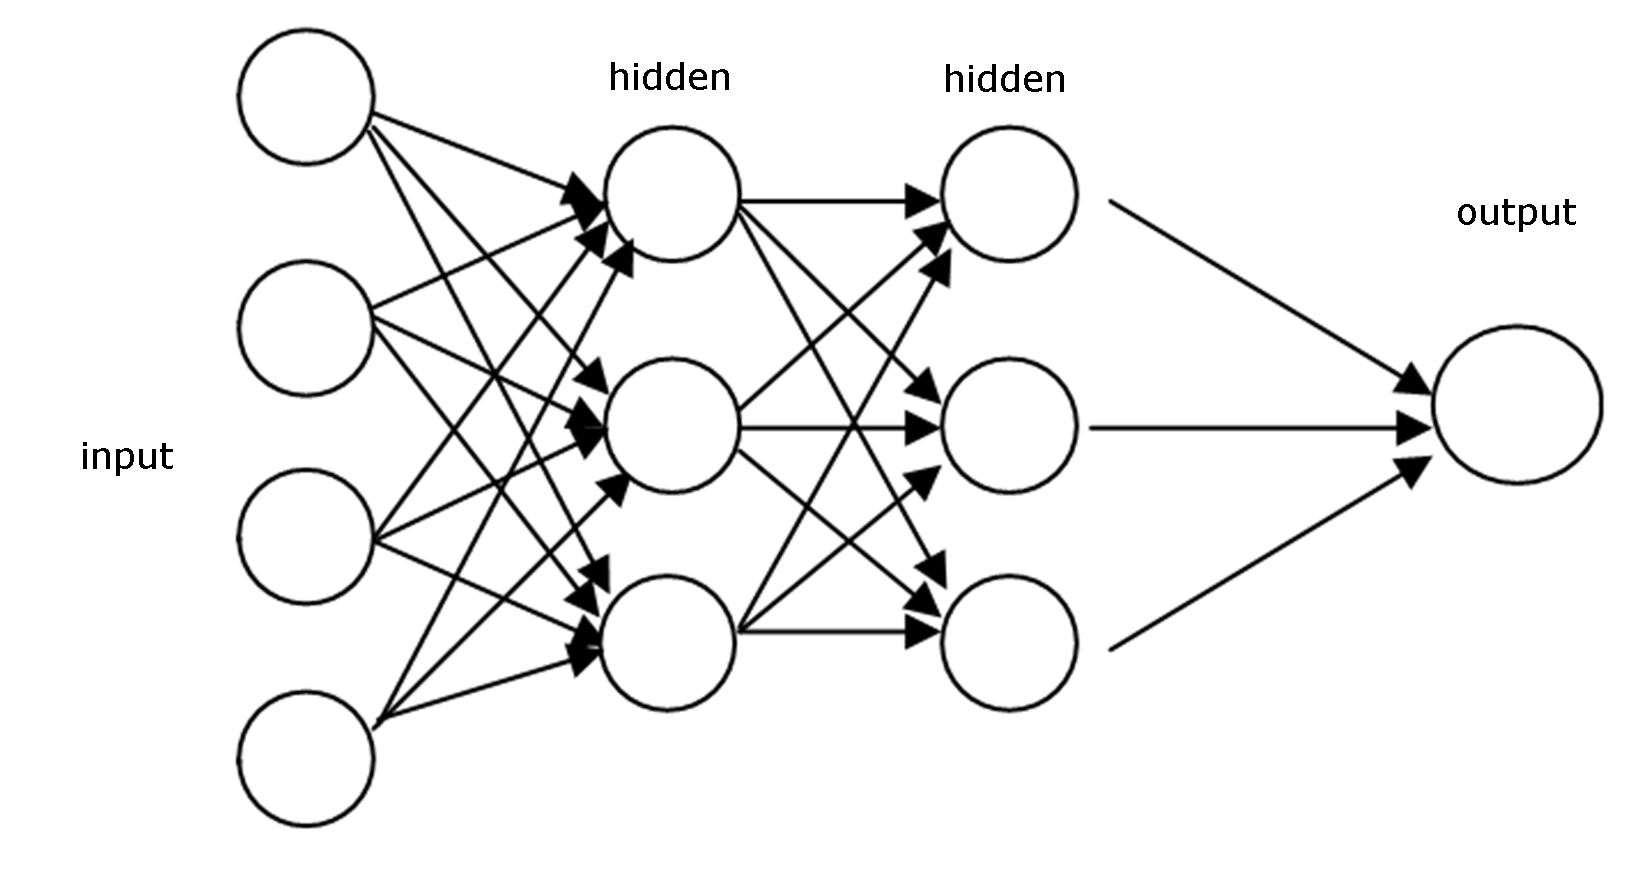
\includegraphics[width=0.8\linewidth]{images/feedforward_structure.png}
    \caption{Structure of a Feedforward Neural Network}
    \label{fig:feedforward_structure}
\end{figure}

Each neuron in a Feedforward Neural Network is a computational unit that applies a weighted sum of its inputs, adds a bias, and passes the result through an activation function. Mathematically, this process can be expressed as:
\[
y = f\left(\sum_{i=1}^{n} w_i x_i + b\right)
\]
where:

- \(y\) is the neuron's output,

- \(x_i\) are the inputs,

- \(w_i\) are the weights associated with the inputs,

- \(b\) is the bias term,

- \(f\) is the activation function (e.g., Sigmoid, ReLU, or Tanh).


A Feedforward Neural Network consists of three main types of layers:

1. Input Layer: This layer receives the input data and serves as the network's entry point. Each node in this layer represents a feature of the input data.

2. Hidden Layers: These layers perform the bulk of the computation in the network. Each hidden layer applies a transformation to the data using weights, biases, and activation functions. The number of hidden layers and their respective sizes define the network's capacity to model complex functions.

3. Output Layer: This layer produces the network's predictions. For classification tasks, the output layer typically applies a Softmax activation function to generate probabilities for each class.

\begin{figure}[h!]
    \centering
    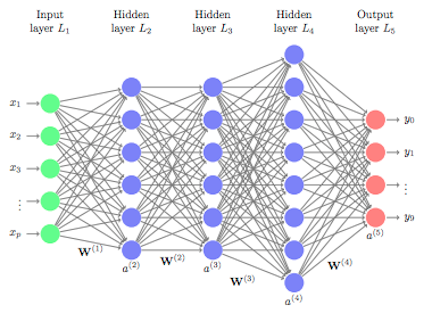
\includegraphics[width=1\linewidth]{images/feedforward_workflow.png}
    \caption{Workflow of a Feedforward Neural Network}
    \label{fig:feedforward_workflow}
\end{figure}

The workflow of a Feedforward Neural Network can be summarized as follows. First, during forward propagation, the input data passes through the network layer by layer. Each layer performs a linear transformation on the inputs, followed by the application of a non-linear activation function. The final layer then generates predictions, which can be probabilities in the case of classification tasks or continuous values for regression tasks.

Next, the loss calculation step measures the difference between the predicted outputs and the true labels using a loss function. 

Following this, backpropagation is performed to update the network's parameters. In this step, the gradient of the loss function with respect to each weight and bias is computed using the chain rule. These gradients are propagated backward through the network, allowing the parameters to be adjusted to minimize the loss.

Finally, during optimization, an algorithm such as Gradient Descent or Adam uses the calculated gradients to iteratively update the weights and biases, thereby improving the network's performance and enabling it to learn from the data.

Feedforward Neural Networks are foundational in deep learning, commonly used for structured data and simple tasks. While not ideal for large-scale image classification due to their lack of specialized operations, they are included here to observe their behavior and compare with more advanced architectures.

\subsection{Convolutional Neural Networks}
%To understand the structure and function of a Convolutional Neural Network (CNN), it is essential first to grasp the basic concept of a Neural Network (NN). A Neural Network consists of an input layer, one or more hidden layers, and an output layer. The input layer receives training data, while the hidden layers perform the computational processes that lead to the output layer, which produces the results. The next figure illustrates the structure of a Neural Network, showcasing the connections between layers, where each connection is associated with a weight. These weights represent the "cost" or influence of one neuron on another.

%\begin{figure}[h!]
%    \centering
%    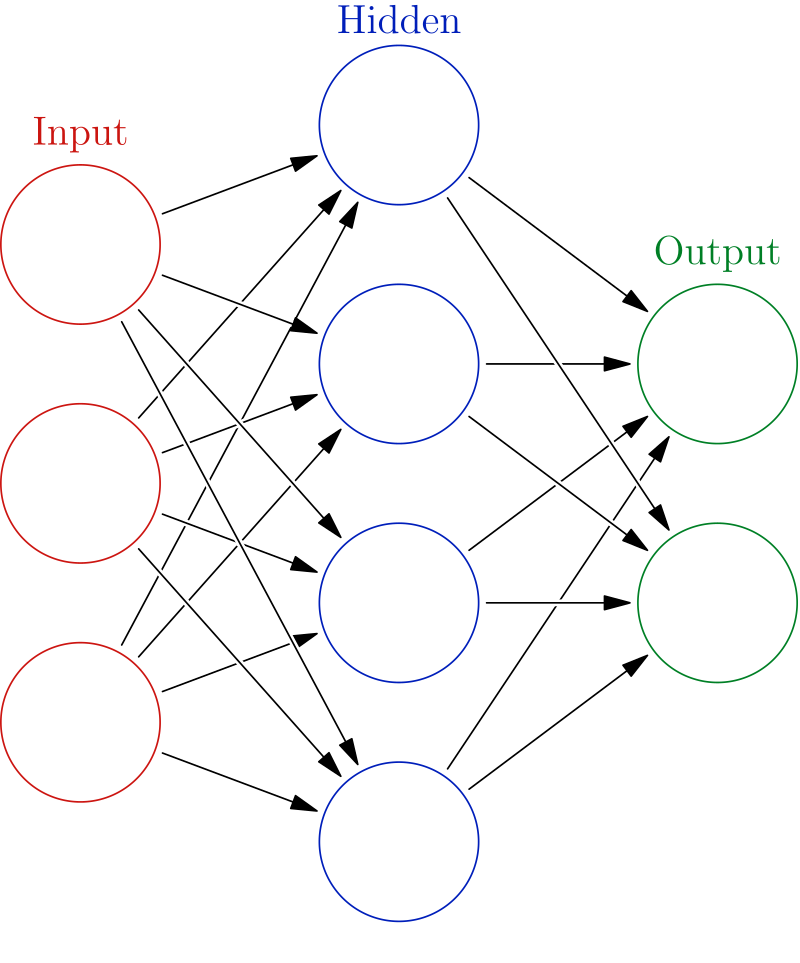
\includegraphics[width=0.75\linewidth]{images/NN_struture.png}
%    \caption{NN Struture}
%    \label{fig:enter-label}
%\end{figure}

%However, traditional Neural Networks face significant challenges when 
Traditional Neural Networks such as FNNs face significant challenges when applied to image data. For instance, an image of size 100×100×3 (height, width, and color channels) contains 30,000 features per image. If every feature is connected to all neurons in the next layer, the model becomes computationally prohibitive and prone to overfitting due to insufficient training data. And to worsen this, they lack specific mechanisms to capture the spatial relationships between image pixels. These limitations make standard Neural Networks unsuitable for complex image classification tasks.

CNNs overcome these limitations by employing convolution, a specialized operation designed to efficiently process image data. Convolution is mathematically defined as the sum of element-wise products between two matrices—a filter and a segment of the input image. This process is illustrated in Figure \ref{fig:conv_process}.

\begin{figure}[h!]
    \centering
    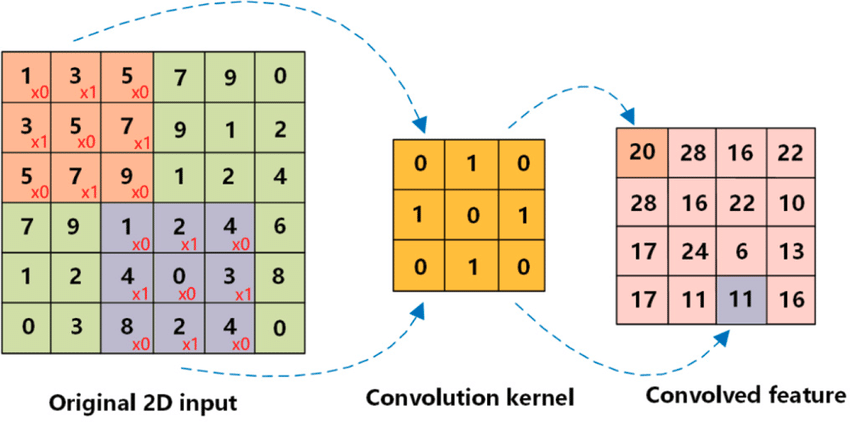
\includegraphics[width=1\linewidth]{images/convolution_process.png}
    \caption{Convolution Process}
    \label{fig:conv_process}
\end{figure}

Filters are fundamental to CNNs, acting as templates for detecting specific features such as edges, textures, or patterns within the input image. As a filter is convolved across the image, it generates a feature map that highlights regions closely matching the filter's pattern. The dimensions of the feature map are determined by the formula:
\[
(n - f + 1) \times (n - f + 1)
\]
where \(n \space = \space  n \times n \) is the input image size, and \( f \space = \space f \times f \) is the filter size.

One challenge of convolution is that it reduces the image size with each operation, potentially discarding valuable edge and corner information. To mitigate this, padding is used. Padding adds extra layers of pixels around the image’s borders, preserving edge and corner details during convolution. 
\begin{figure}[h!]
    \centering
    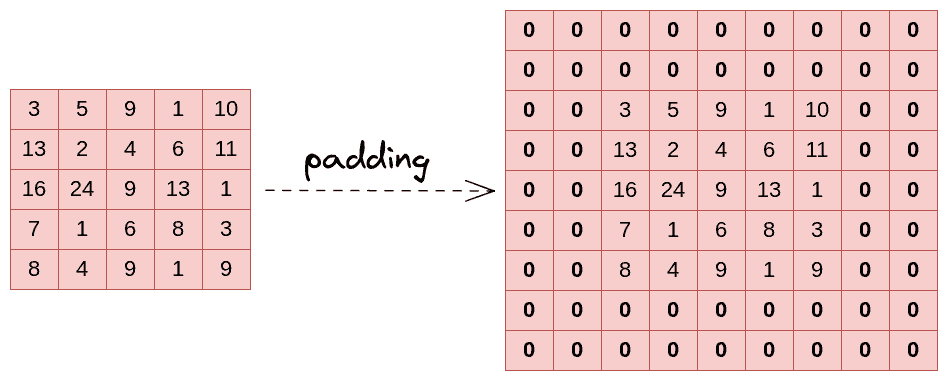
\includegraphics[width=1\linewidth]{images/padding.png}
    \caption{Padding}
    \label{fig:enter-label}
\end{figure}


Another critical CNN component is the pooling layer, which summarizes feature maps by reducing their spatial dimensions. This compression minimizes the number of parameters, making the model more robust and less sensitive to the exact positions of features. In this study, max pooling is employed, selecting the maximum value from each sub-matrix of the feature map. This technique ensures that the most prominent feature in each region is retained, as shown in the next figure.

\begin{figure}[h!]
    \centering
    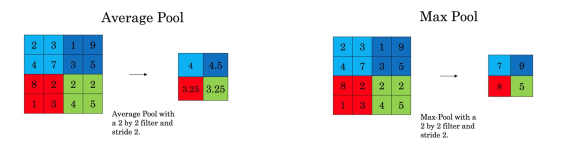
\includegraphics[width=1\linewidth]{images/Pooling.png}
    \caption{Pooling layer}
    \label{fig:enter-label}
\end{figure}


A CNN performs multiple cycles of convolution and pooling to extract hierarchical features from the input image. After these layers, the resulting feature maps are flattened into a one-dimensional vector. This flattened vector serves as the input to a fully connected layer, where the process continues like a standard Neural Network, leading to the final classification output.

\begin{figure}[h!]
    \centering
    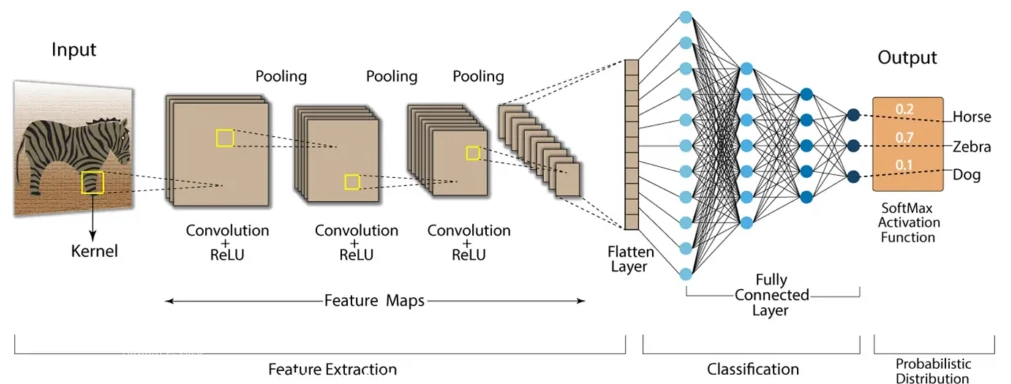
\includegraphics[width=1\linewidth]{images/CNN_example.png}
    \caption{CNN Structure}
    \label{fig:enter-label}
\end{figure}

By combining convolution, pooling, and fully connected layers, CNNs effectively reduce computational requirements and improve accuracy for tasks like image classification, making them an ideal choice for this study.



\subsection{DenseNet}
DenseNet, short for Densely Connected Convolutional Network, is an advanced architecture for deep learning that aims to address some of the limitations of traditional CNNs. Introduced to enhance gradient flow and improve parameter efficiency, DenseNet achieves this by ensuring direct connections between each layer and all subsequent layers, as illustrated in the figure below.

\begin{figure}[h!]
    \centering
    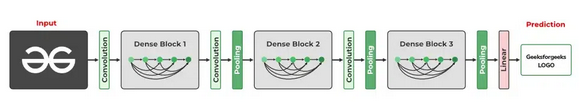
\includegraphics[width=1\linewidth]{images/dense_net_arquitetura.png}
    \caption{Architecture of DenseNet}
    \label{fig:enter-label}
\end{figure}

In DenseNet, every layer receives the feature maps of all preceding layers as input and passes its feature maps to all subsequent layers. This approach contrasts with traditional CNNs, where layers are connected sequentially. DenseNet’s dense connectivity can be mathematically represented as:
\[
x_l = H_l([x_0, x_1, ..., x_{l-1}])
\]

- \(x_l\) represents the output of the \(l\)-th layer.

- \(H_l\) denotes the composite function (e.g., Batch Normalization, ReLU, and Convolution).

- \([x_0, x_1, ..., x_{l-1}]\) represents the concatenation of the feature maps from all preceding layers.

This dense connectivity pattern significantly reduces redundancy, promotes feature reuse, and alleviates the vanishing gradient problem.



DenseNet introduces transition layers to manage the model's size and reduce the spatial dimensions of feature maps. These layers consist of Batch Normalization, a \(1 \times 1\) convolutional operation, and \(2 \times 2\) average pooling. The transition layers ensure that the network remains compact and computationally efficient while preserving important features.

\begin{figure}[h!]
    \centering
    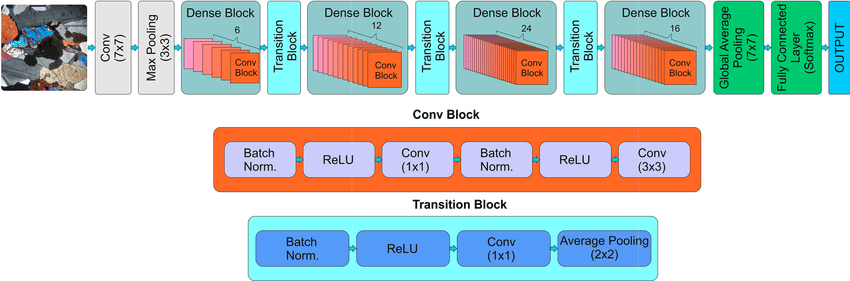
\includegraphics[width=1\linewidth]{images/DenseNet_transition.png}
    \caption{DenseNet Transition Layer}
    \label{fig:densenet_transition}
\end{figure}

Dense blocks are the core components of DenseNet, where the dense connectivity occurs. Within a dense block, each layer has access to the feature maps of all previous layers, promoting efficient feature propagation and reuse. Let \(k\) denote the growth rate, which determines the number of feature maps each layer contributes. The feature map count in a dense block grows linearly with the number of layers.

The output of a dense block with \(L\) layers can be expressed as:
\[
\text{Output feature maps} = k \cdot L
\]
where \(k\) is a hyperparameter chosen based on the model's complexity requirements.


\begin{figure}[h!]
    \centering
    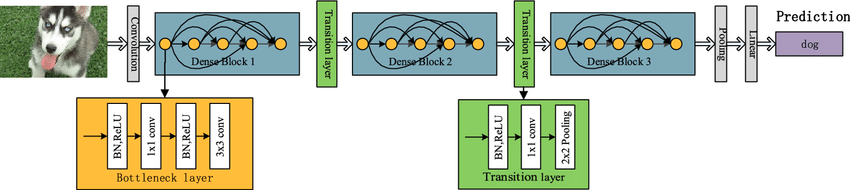
\includegraphics[width=1\linewidth]{images/DenseNet_workflow.png}
    \caption{DenseNet Example}
    \label{fig:densenet_workflow}
\end{figure}

The workflow of DenseNet combines dense blocks and transition layers to achieve an efficient and compact model structure. 

1. Input Layer: The input image is first processed by an initial convolutional layer to extract basic features.

2. Dense Block: Each dense block performs iterative feature extraction, where each layer has direct access to all previous layers' feature maps. This promotes feature reuse and minimizes redundancy.

3. Transition Layer: Between dense blocks, transition layers reduce the spatial dimensions and feature map count, ensuring computational efficiency and controlling model size.

4. Final Classification: After passing through a series of dense blocks and transition layers, the feature maps are global average pooled, flattened, and fed into a fully connected layer for the final classification output.

This structured workflow ensures that DenseNet achieves superior gradient flow, efficient parameter use, and excellent feature extraction capabilities, making it a powerful architecture for tasks like image classification, making them an ideal choice for this study.


\subsection{Data Augmentation and Hyperparameter Tuning}

To enhance the performance and generalization of the machine learning models, this study employs two critical techniques: data augmentation and hyperparameter tuning.

\subsubsection{Data Augmentation}
Data augmentation is applied to artificially increase the diversity and size of the training dataset, mitigating overfitting and improving the models' ability to generalize to unseen data. This is achieved by applying transformations such as random rotations, flips, zooming, cropping, and changes in brightness or contrast to the input images. These transformations introduce variability while preserving the semantic meaning of the data, ensuring that the models learn robust features rather than overfitting to specific patterns in the original dataset.

\begin{figure}[h!]
    \centering
    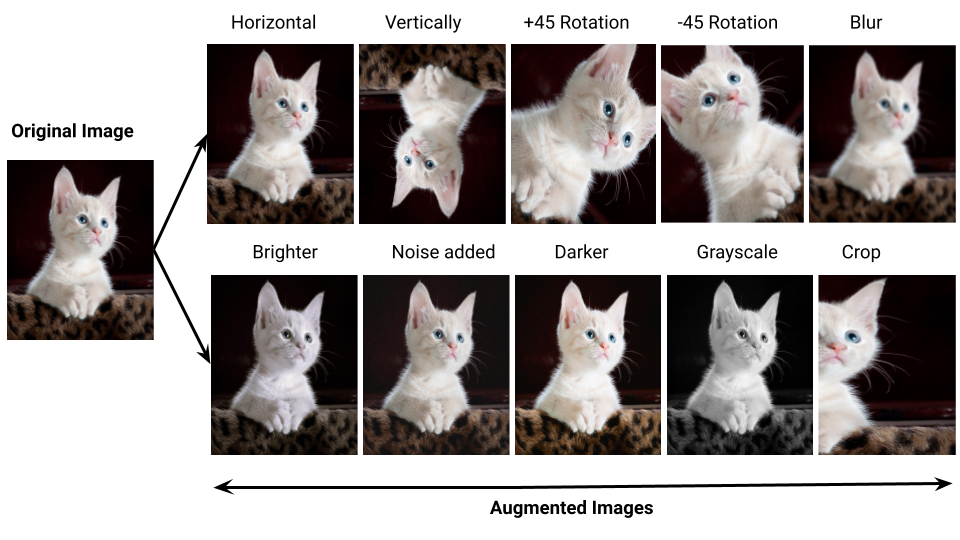
\includegraphics[width=0.9\linewidth]{images/data_augmentation.png}
    \caption{Data Augmentation examples}
    \label{fig:enter-label}
\end{figure}

\subsubsection{Hyperparameter Tuning}
Hyperparameter tuning involves systematically optimizing the key parameters that govern the training process and architecture of the models. Examples of hyperparameters include the learning rate, batch size, number of layers, number of neurons per layer, and dropout rates. This process is conducted using techniques like grid search or random search to identify the optimal combination of hyperparameters that maximize the models' performance on the validation dataset. Tuning ensures that the models achieve a balance between underfitting and overfitting, leading to better overall accuracy and generalization.

\hfill


By integrating data augmentation and hyperparameter tuning into the training workflow, the implemented models are better equipped to handle the challenges of scene image classification, yielding improved accuracy and robustness in their predictions. At the end of the study, the results will be compared across various configurations, including baseline models without augmentation or tuning, models with data augmentation, and models with optimized hyperparameters, to evaluate the impact of these techniques on performance.



\subsection{Model Evaluation: Confusion Matrix and Classification Metrics}
The evaluation of the models will be carried out using the confusion matrix, which provides a detailed view of the model’s correct and incorrect predictions for each class (e.g., road, forest, etc.). In addition, classification metrics including \textit{accuracy}, \textit{precision}, \textit{recall}, and \textit{F1-score} will be calculated. These metrics are essential for assessing the effectiveness of the model in differentiating between various scene types.

\subsubsection{Confusion Matrix}
A confusion matrix is a table that
indicates the mistakes and successes of your model, comparing to the expected result, the layout of a confusion matrix in present on the next figure. We will utilize to compute the confusion matrix, which is the sklearn function of confusion matrix.

\begin{figure}[h!]
    \centering
    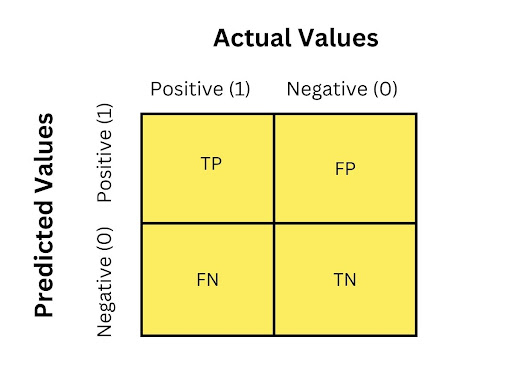
\includegraphics[width=0.75\linewidth]{images/confusion_matrix.png}
    \caption{Confusion Matrix}
    \label{fig:enter-label}
\end{figure}


\subsubsection{Precision}
Precision score, a vital metric in evaluating classification models, measures the ratio of true positive predictions to the total number of positive predictions made by the model. It provides insight into the model’s ability to correctly identify relevant instances from all instances predicted as positive.
The precision score is calculated as:
\[Precision=\frac{True Positives (TP)}{True Positives (TP)+False Positives (FP)}\]

\subsubsection{Recall (Sensitivity)}
Recall score, also known as sensitivity or true positive rate, gauges the model’s ability to correctly identify all relevant instances from the total number of actual positive instances in the dataset.
Its formula is the following:
\[Recall=\frac{True Positives (TP)}{True Positives (TP)+False Negatives (FN)}\]

\subsubsection{F1-Score}
The F1 score, a harmonic mean of precision
and recall, provides a balanced assessment of a model’s
performance. It combines both precision and recall into a
single metric, making it useful for evaluating models with imbalanced class distributions.
\[F1Score=2 \times \frac{Precision*Recall}{Precision+Recall}\]

\subsubsection{Accuracy}
Accuracy is the proportion of correct predictions (both true positives and true negatives) to the total number of predictions made. It represents the overall correctness of the model's predictions. It is especially usefull when the dataset is balanced.
\[Accuracy= \frac{True Positives (TP)\times True Negatives (TN)}{Total Predictions}\]


\subsubsection{Training Loss}
Training loss quantifies how well the model fits the training data by calculating the difference between predicted and actual values. It is computed using a loss function such as cross-entropy for classification or mean squared error for regression. A lower loss means better model predictions. The goal during training is to minimize loss, but low training loss doesn’t always imply good generalization—overfitting can occur if the model is too closely fit to the training data.

\subsubsection{ROC curve graph}
The ROC (Receiver Operating Characteristic) curve is a graphical representation used to evaluate the performance of binary classifiers. It shows the trade-off between the True Positive Rate (TPR) and False Positive Rate (FPR) as the classification threshold varies. TPR is also known as sensitivity, and FPR is 1 - specificity.

% True Positive Rate (TPR)
\[
\text{TPR} = \frac{\text{True Positives (TP)}}{\text{True Positives (TP)} + \text{False Negatives (FN)}}
\]

% False Positive Rate (FPR)
\[
\text{FPR} = \frac{\text{False Positives (FP)}}{\text{False Positives (FP)} + \text{True Negatives (TN)}}
\]

The curve is plotted with the False Positive Rate (FPR) on the x-axis and the True Positive Rate (TPR) on the y-axis. Each point on the curve corresponds to a different threshold for classifying positive and negative outcomes.

\begin{figure}[h!]
    \centering
    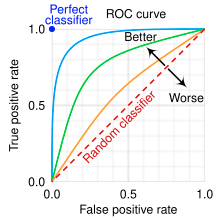
\includegraphics[width=0.75\linewidth]{images/roc.png}
    \caption{ROC Example}
    \label{fig:enter-label}
\end{figure}

The Area Under the Curve (AUC) summarizes the model's overall performance. A perfect classifier has an AUC of 1, while a random classifier has an AUC of 0.5. The ROC curve helps in selecting an optimal threshold for balancing sensitivity and specificity according to the specific requirements of the problem.


\section{Data Visualization}
\label{sec:Data Visualization}
\subsection{Dataset Description}
The Intel Image Classification dataset provides a comprehensive collection of images depicting various scenes, serving as a robust foundation for training and evaluating scene classification models. This dataset comprises approximately 25,000 images, each categorized into one of six scene types: buildings, forest, glacier, mountain, sea, and street.

\begin{figure}[h!]
    \centering
    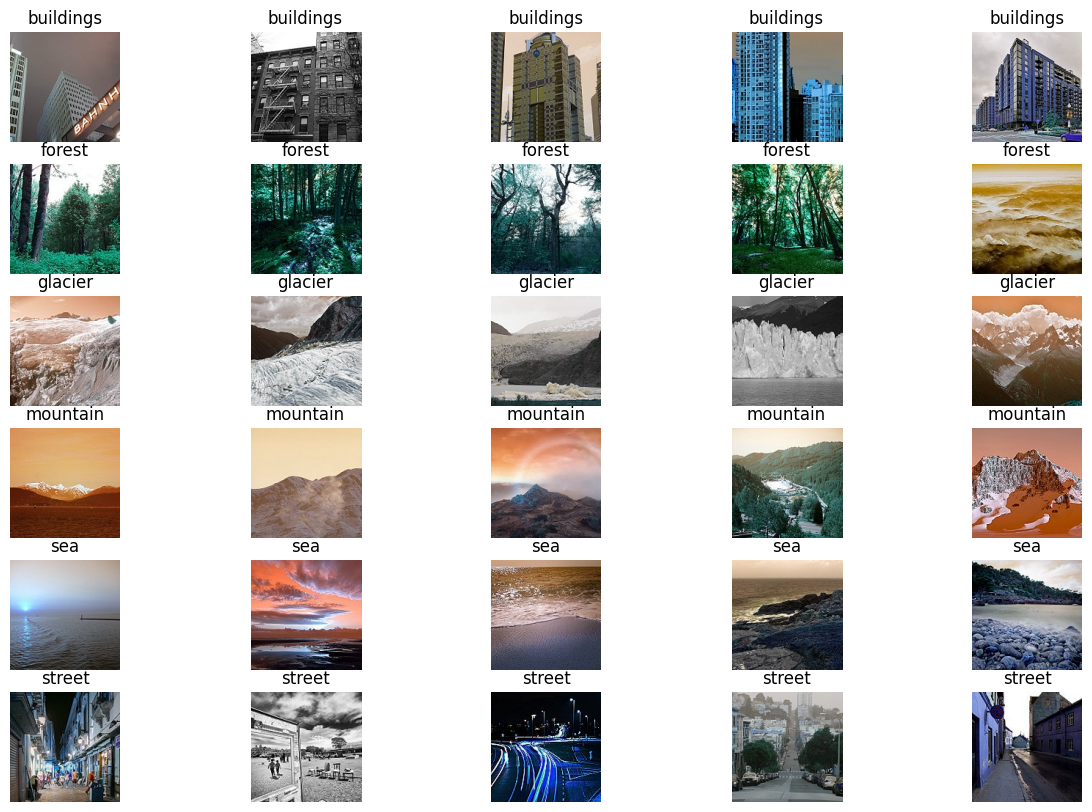
\includegraphics[width=1\linewidth]{images/conjunto_dados.png}
    \caption{Examples of scenes}
    \label{fig:Examples-of-scenes}
\end{figure}

The dataset is pre-divided into three subsets: training, testing, and prediction. Specifically, it includes around 14,000 images for training, 3,000 images for testing, and 7,000 images for prediction. This structured division facilitates streamlined experimentation, ensuring that models can be effectively trained on a substantial dataset and rigorously evaluated on separate, unseen data.

With six distinct classes, the dataset poses a challenging multi-class classification problem. By leveraging the complete training set to develop the model and the testing set for performance evaluation, the goal is to achieve accurate categorization of images across all six scene types. This dataset's diversity and size make it an ideal resource for advancing research in scene image classification.

\subsection{Exploratory Analysis}
The data distribution in both the training and test datasets is uniform, with each class equally represented, as illustrated in  \ref{fig:hist} and \ref{fig:pie}. This uniformity minimizes variance among classes, providing an ideal foundation for efficient model training without introducing bias.

\begin{figure}[h!]
    \centering
    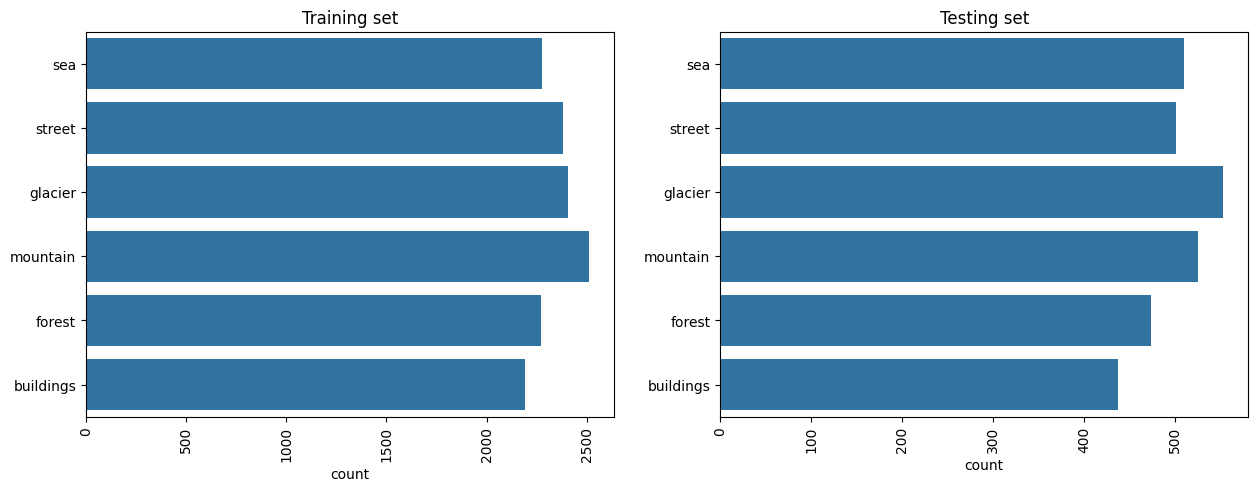
\includegraphics[width=1\linewidth]{images/hist_test_x_train.png}
    \caption{Distribution of training and testing data}
    \label{fig:hist}
\end{figure}
\begin{figure}[h!]
    \centering
    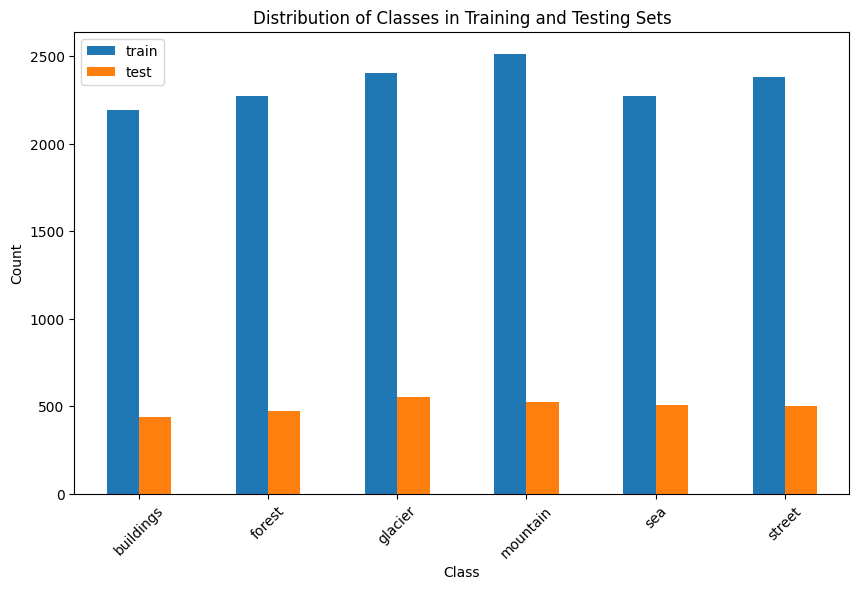
\includegraphics[width=0.75\linewidth]{images/train_vs_test.png}
    \caption{Distribution of training and testing data}
    \label{fig:enter-label}
\end{figure}
\begin{figure}[h!]
    \centering
    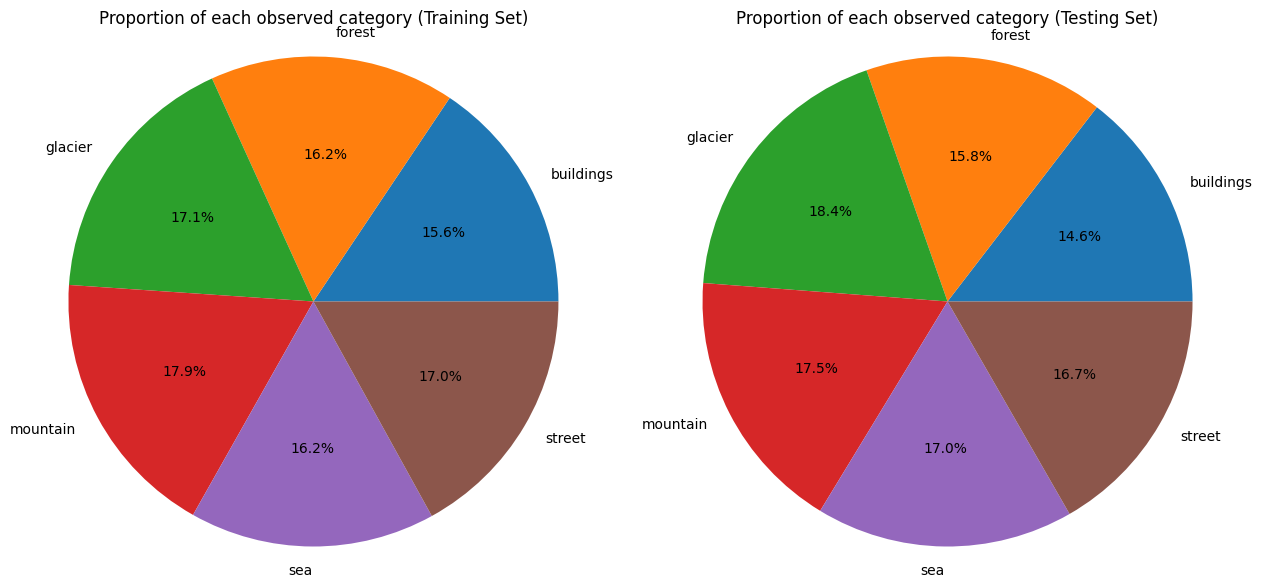
\includegraphics[width=1\linewidth]{images/pie_test_x_train.png}
    \caption{Distribution chart of training and testing data}
    \label{fig:pie}
\end{figure}


A balanced dataset ensures that the model receives equitable exposure to all classes, enabling balanced parameter updates during training. This leads to improved learning efficiency and enhances the model’s ability to deliver reliable and fair predictions across all classes. Such uniformity is critical for achieving robust performance in multi-class classification tasks.

\subsection{Data Prerocessing}

For data preprocessing, once the data is balanced across all classes in both the training and test sets, as outlined in the previous section, the primary preprocessing step is normalization.

In the raw dataset, pixel values range from 0 to 255, a wide range that can adversely impact model training by introducing numerical instability and slower convergence. To address this, each pixel value is scaled by dividing it by 255, effectively normalizing the range to [0, 1]. This transformation ensures consistent input data, enhancing the model's training efficiency and stability while improving scalability and overall performance.

By normalizing the pixel values, the model can focus on learning meaningful patterns rather than being affected by the magnitude of the raw input values, leading to better generalization and more reliable predictions.
\section{Results}

In this section, we present the results obtained throughout the development of the work, detailing the different approaches and techniques applied for image classification in the Intel Image Classification dataset.

Initially, we used a basic convolutional neural network (CNN), as presented in class, to establish an initial baseline. Next, we introduced the data augmentation technique to increase the diversity of the dataset and improve the model's performance, conducting training for 10 epochs.

Subsequently, we explored feedforward neural networks (FNNs), testing different combinations of hyperparameters. We continued the experiment by applying another CNN, again varying its hyperparameters. Both FNN and CNNs were trained for 30 epochs using data augmentation techniques.

Finally, we implemented the DenseNet architecture, a state-of-the-art network, and performed two experiments: one without data augmentation and another using the technique to analyze the impacts of this approach on an advanced model, conducting training for 30 epochs.

\subsection{CNN Model Class}

The first version of our Convolutional Neural Network (CNN) was designed with a straightforward architecture aimed at establishing a baseline performance metric. The model includes three convolutional layers, each followed by a max-pooling layer, with a fully connected dense layer and a dropout layer for regularization before the output layer. The specific architecture is as follows:

\begin{table}[H]
\centering
\caption{Architecture of the CNN Model}
\begin{tabular}{|l|c|c|}
\hline
\textbf{Layer (Type)}          & \textbf{Output Shape} & \textbf{Parameters} \\ \hline
Conv2D                         & (None, 148, 148, 32)  & 896                 \\ \hline
MaxPooling2D                   & (None, 74, 74, 32)    & 0                   \\ \hline
Conv2D                         & (None, 72, 72, 64)    & 18,496              \\ \hline
MaxPooling2D                   & (None, 36, 36, 64)    & 0                   \\ \hline
Conv2D                         & (None, 34, 34, 128)   & 73,856              \\ \hline
MaxPooling2D                   & (None, 17, 17, 128)   & 0                   \\ \hline
Flatten                        & (None, 36992)         & 0                   \\ \hline
Dense                          & (None, 128)           & 4,735,104           \\ \hline
Dropout                        & (None, 128)           & 0                   \\ \hline
Dense                          & (None, 6)           & 774           \\ \hline
\hline
\textbf{Total params:}        & \multicolumn{2}{l|}{4,829,126}              \\ \hline
\textbf{Trainable params:}    & \multicolumn{2}{l|}{4,829,126}              \\ \hline
\textbf{Non-trainable params:} & \multicolumn{2}{l|}{0}                      \\ \hline
\end{tabular}
\label{tab:cnn_architecture}
\end{table}


The model was compiled using the Adam optimizer with a default learning rate of 0.001. The Adam optimizer is well suited for this task due to its adaptive learning rate capabilities.
The loss function used is ”categorical crossentropy”, which is appropriate for multiclass classification problems, and the performance metric tracked during training was accuracy.
The performance of the first CNN was evaluated using training, validation, and test datasets. The model demonstrated a high accuracy on the training data but showed a significant drop in accuracy on the validation and test data, indicating potential overfitting.

The next figure provides a visual representation of the accuracy and loss trends for both training and validation data across the \textbf{10 epochs}, offering insights into the model's learning dynamics.
The model achieved higher accuracy on the training data compared to the validation and test data. This discrepancy suggests potential overfitting, where the model performs well on the data it has seen but struggles to generalize effectively to unseen data. This behavior is further corroborated by the loss values recorded during training and validation, which highlight the challenges in maintaining consistency across the dataset.

\begin{figure}[h!]
    \centering
    \begin{subfigure}[t]{0.45\textwidth} % Tamanho de cada subfigura
        \centering
        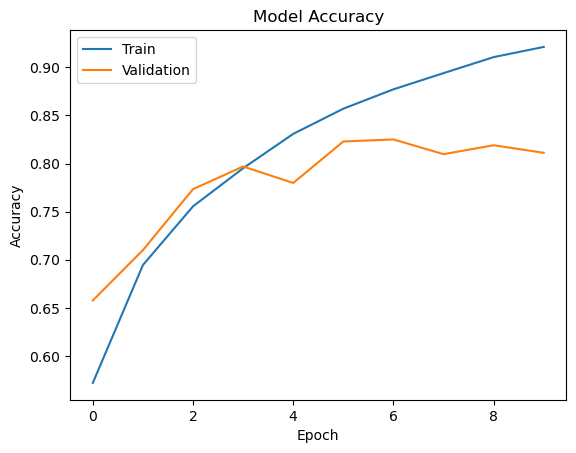
\includegraphics[width=\textwidth]{images/model_class_accuracy.png}
        \caption{Train vs Validation Accuracy}
        \label{fig:subfig1}
    \end{subfigure}
    \hfill
    \begin{subfigure}[t]{0.45\textwidth}
        \centering
        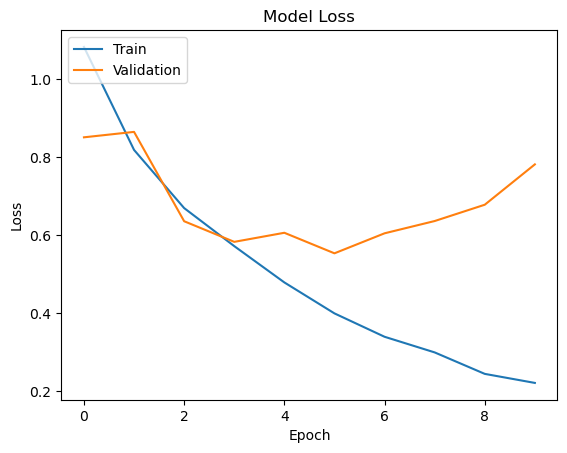
\includegraphics[width=\textwidth]{images/model_class_loss.png}
        \caption{Train vs Validation Loss}
        \label{fig:subfig2}
    \end{subfigure}
    \caption{Accuracy and Loss for the First Model}
    \label{fig:images}
\end{figure}

The graphs reveal that while the training accuracy consistently improves and the training loss decreases, the validation accuracy stagnates after the initial epochs, and the validation loss increases. This pattern further reinforces the indication of overfitting.

To gain a deeper understanding of the model's performance, we generated the confusion matrix for the test data and calculated the precision, recall, and F1-score, providing a more comprehensive evaluation of the model's effectiveness across different classes.

\begin{figure}[H]
    \centering
    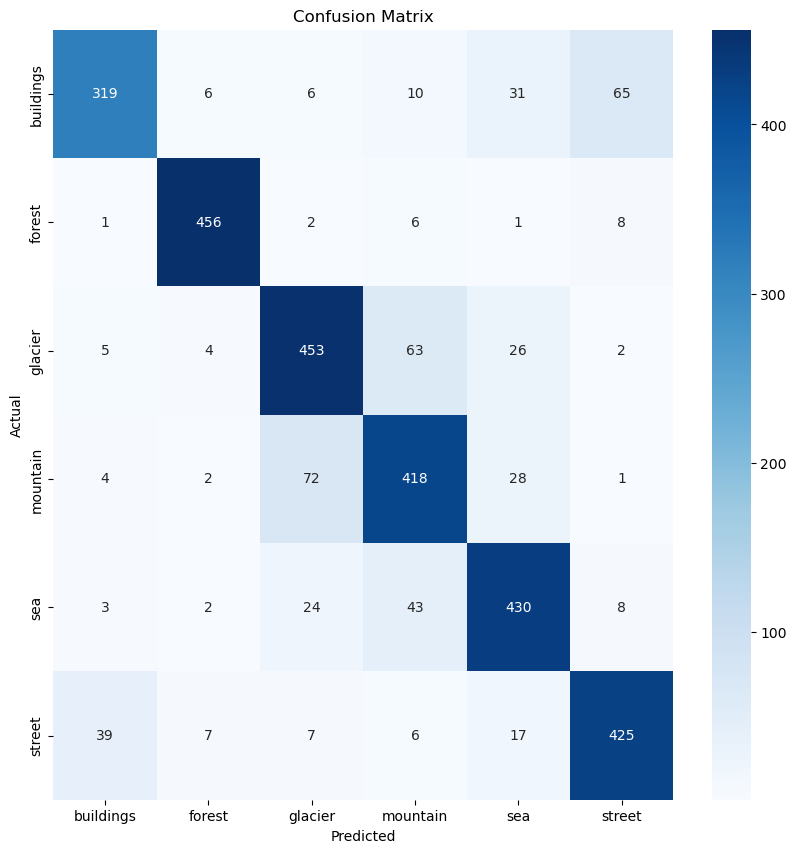
\includegraphics[width=1\linewidth]{images/model_aulas_confusion.png}
    \caption{Model Confusion Matrix}
    \label{fig:enter-label}
\end{figure}

\begin{figure}[H]
    \centering
    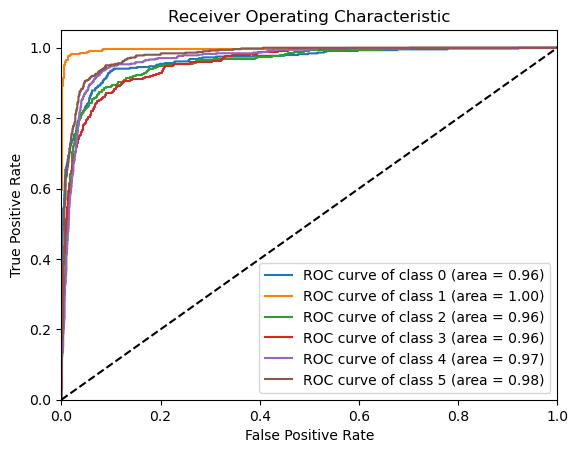
\includegraphics[width=1\linewidth]{images/modelo_aula_roc.png}
    \caption{Roc Curve}
    \label{fig:rocincial}
\end{figure}

\begin{table}[H]
    \centering
    \caption{Model Test Evaluation Metrics} 
    \begin{tabular}{||c|c|c|c|c||} 
        \hline
        Accuracy & F1 Score & Recall & Precision \\
        \hline\hline
        0.834 & 0.834 & 0.834 & 0.835 \\
        \hline
    \end{tabular}
    \label{tab:tab_LogReg}
\end{table}

Forests (1) are classified very accurately, with the majority of predictions falling in the correct category. Meanwhile, Buildings (0) are often misclassified as Streets (5), with 65 misclassifications, and Streets (5) are sometimes confused with Buildings (0) and Sea (4). On the same note, Mountains (3) and Glaciers (2) frequently get confused with each other, reflecting their visual similarities (72 mountains as glaciers and 63 glaciers as mountains).

The ROC (Receiver Operating Characteristic) curves for the six scene classes provide an overall view of the model’s ability to distinguish between different types of scenery. Each ROC curve plots the true positive rate against the false positive rate, with the Area Under the Curve (AUC) representing the
model’s performance. As it can be seen in Roc Curve, class 1 (forest), had the best AUC Value, while the rest of the scenes came short. 

\subsection{CNN Model Class with Data Augmentation}

This Convolutional Neural Network (CNN) model follows the same architecture as the previous model, but with the addition of data augmentation to enhance the model's ability to generalize. Data augmentation techniques, including random rotations, width and height shifts, zooming, shearing, and horizontal flipping, were applied to the training data. These transformations aim to create a more diverse set of images for training, which helps in reducing overfitting.
\begin{table}[H]
\centering
\caption{Architecture of the CNN Model}
\begin{tabular}{|l|c|c|}
\hline
\textbf{Layer (Type)}          & \textbf{Output Shape} & \textbf{Parameters} \\ \hline
Conv2D                         & (None, 148, 148, 32)  & 896                 \\ \hline
MaxPooling2D                   & (None, 74, 74, 32)    & 0                   \\ \hline
Conv2D                         & (None, 72, 72, 64)    & 18,496              \\ \hline
MaxPooling2D                   & (None, 36, 36, 64)    & 0                   \\ \hline
Conv2D                         & (None, 34, 34, 128)   & 73,856              \\ \hline
MaxPooling2D                   & (None, 17, 17, 128)   & 0                   \\ \hline
Flatten                        & (None, 36992)         & 0                   \\ \hline
Dense                          & (None, 128)           & 4,735,104           \\ \hline
Dropout                        & (None, 128)           & 0                   \\ \hline
Dense                          & (None, 6)           & 774           \\ \hline
\hline
\textbf{Total params:}        & \multicolumn{2}{l|}{4,829,126}              \\ \hline
\textbf{Trainable params:}    & \multicolumn{2}{l|}{4,829,126}              \\ \hline
\textbf{Non-trainable params:} & \multicolumn{2}{l|}{0}                      \\ \hline
\end{tabular}
\label{tab:cnn_architecture}
\end{table}

\begin{figure}[H]
    \centering
    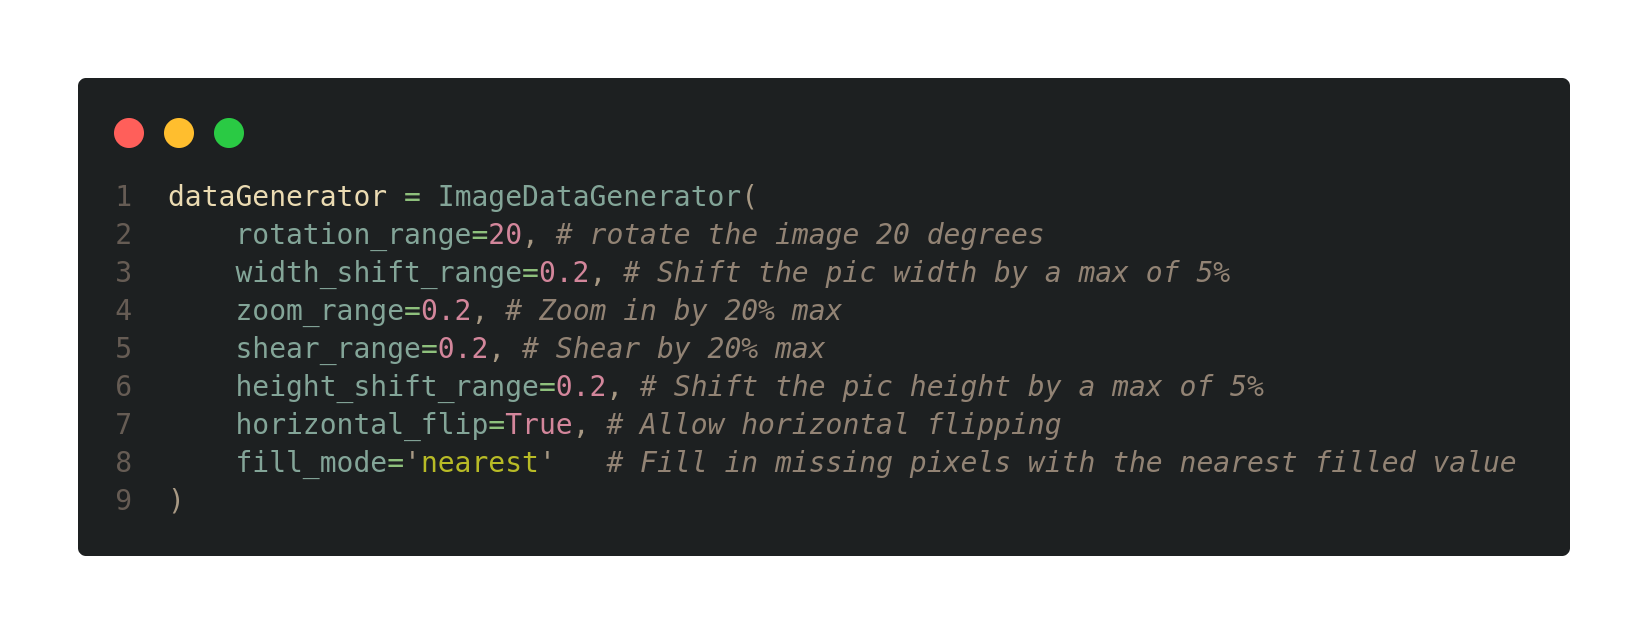
\includegraphics[width=1\linewidth]{images/modelo_aulas_dataaug.png}
    \caption{Data Augmentation Applied}
    \label{fig:enter-label}
\end{figure}

The next figure provides a visual representation of the accuracy and loss trends for both training and validation data across the \textbf{10 epochs}, offering insights into the model's learning dynamics.

\begin{figure}[H]
    \centering
    \begin{subfigure}[t]{0.45\textwidth} % Tamanho de cada subfigura
        \centering
        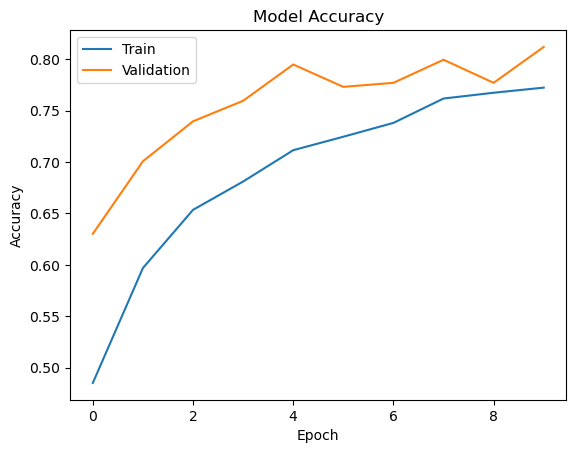
\includegraphics[width=\textwidth]{images/modelo_aula_accuracy_dataaug.png}
        \caption{Train vs Validation Accuracy}
        \label{fig:subfig1}
    \end{subfigure}
    \hfill
    \begin{subfigure}[t]{0.45\textwidth}
        \centering
        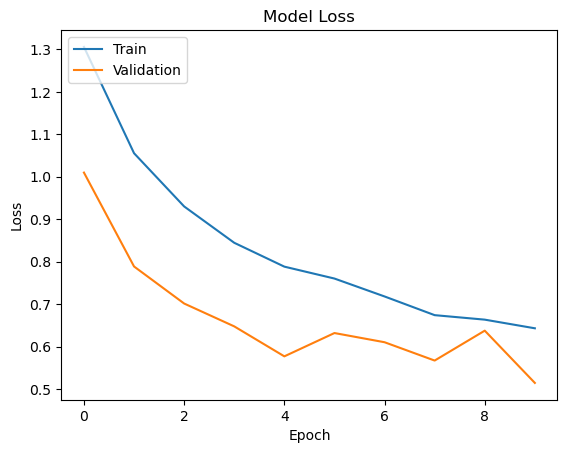
\includegraphics[width=\textwidth]{images/modelo_aula_loss_dataaug.png}
        \caption{Train vs Validation Loss}
        \label{fig:subfig2}
    \end{subfigure}
    \caption{Accuracy and Loss for the First Model with Data Augmentation}
    \label{fig:images}
\end{figure}

The graphs reveal that, unlike the model without data augmentation, the discrepancy between training and validation performance is no longer evident. The training accuracy consistently improves while the validation accuracy closely follows, remaining slightly higher throughout the epochs. Additionally, the training and validation loss curves align more closely, indicating that the model benefits from the data augmentation, reducing overfitting and generalizing better to unseen data.

To gain a deeper understanding of the model's performance, we generated the confusion matrix for the test data and calculated the precision, recall, and F1-score, providing a more comprehensive evaluation of the model's effectiveness across different classes.

\begin{figure}[H]
    \centering
    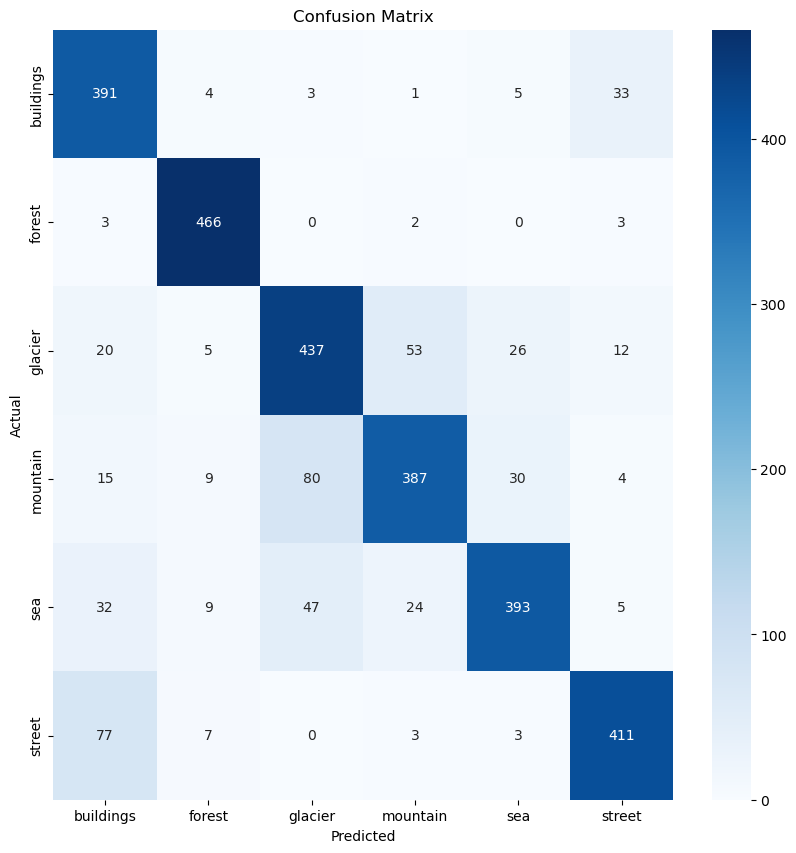
\includegraphics[width=1\linewidth]{images/modelos_aula_confusion_dataaug.png}
    \caption{Model Confusion Matrix}
    \label{fig:enter-label}
\end{figure}

\begin{figure}[H]
    \centering
    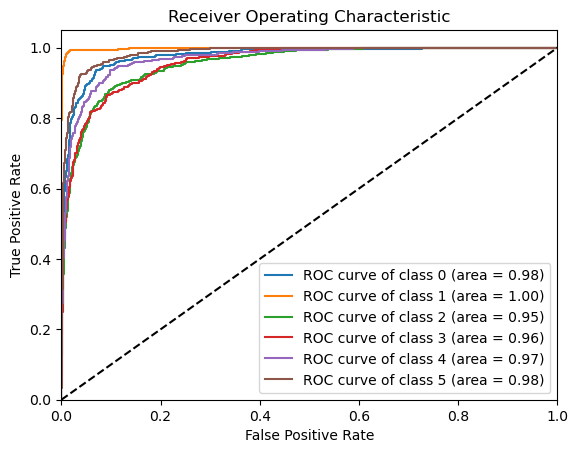
\includegraphics[width=1\linewidth]{images/modelo_aula_roc_dataaug.png}
    \caption{Roc Curve}
    \label{fig:rocincial}
\end{figure}

\begin{table}[H]
    \centering
    \caption{Model Test Evaluation Metrics} 
    \begin{tabular}{||c|c|c|c|c||} 
        \hline
        Accuracy & F1 Score & Recall & Precision \\
        \hline\hline
        0.823 & 0.828 & 0.829 & 0.832 \\
        \hline
    \end{tabular}
    \label{tab:tab_LogReg}
\end{table}


With the inclusion of data augmentation, the model continues to face challenges in distinguishing certain categories. Specifically, Streets (5) are still frequently misclassified as Buildings (0), with 77 instances of such misclassification. Similarly, the confusion between Mountains (3) and Glaciers (2) persists, as well as between Sea (4) and Glaciers (2), reflecting ongoing difficulties in differentiating visually similar categories.

While it was anticipated that data augmentation would lead to improvements in evaluation metrics such as precision, recall, F1-score, and accuracy, the results showed that these metrics remained relatively unchanged. This indicates that although data augmentation helped in diversifying the training data, it did not significantly enhance the model's ability to resolve the inherent challenges of certain class distinctions.

The ROC (Receiver Operating Characteristic) curves for the six scene classes provide a comprehensive overview of the model’s ability to differentiate between various types of scenery. Each curve plots the true positive rate against the false positive rate, with the Area Under the Curve (AUC) indicating the model’s performance.

With data augmentation, the ROC curves improved across most classes, except for class 2 (Glacier), where the AUC value decreased slightly, and in some cases, the values remained unchanged. Notably, class 1 (Forest) continued to demonstrate the best AUC value, showcasing the model's strength in accurately classifying this category. 

\subsection{Feedforward Neural Networks (FNNs)}
Following the CNN Class with Data Augmentation, we explored Feedforward Neural Networks. This FNN approach uses Data Augmentation to techniques which are exhibited in the following image.
\begin{figure}[H]
    \centering
    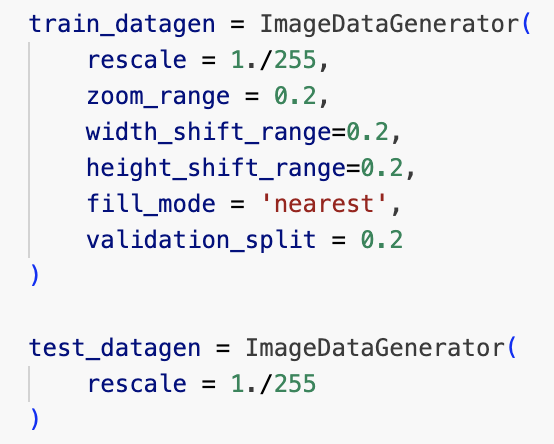
\includegraphics[width=0.5\linewidth]{images/fnn_data_aug.png}
    \caption{Data Augmentation techniques that were used.}
    \label{fig:FNN_data_aug}
\end{figure}
The techniques used include random zooms in or out on the images by up to 20\%, random shifts of the image horizontally and vertically up to 20\%, and a strategy that fills the missing pixels created by zooms and other transformations using the nearest pixel values.

The implemented FNN model includes an input layer, three hidden layers, and an output layer. As with the previous CNN, the model was compiled using the Adam optimizer and the loss function is the "categorical crossentropy".

A grid search approach of hypertuning the model was used. It consisted of trying out different values of the hyperparameters and picking the "model" that gives the best score. This approach was used for balancing computational efficiency and thoroughness in exploring hyperparameter combinations. The hyperparameters that were tuned are the number of neurons per hidden layer and the activation function of the hidden layers. The values experimented of each hyperparameter can be consulted in the table \ref{tab:fnn_hypertuning}.

\begin{table}[H]
\centering
\caption{FNN tuned hyperparameters.}
\begin{tabular}{|l|c|}
\hline
\textbf{Hyperparameter} & \textbf{Values} \\ \hline
Number of neurons per hidden layer & \{25, 50, 100, 200\} \\ \hline
Activation & \{ReLU, Sigmoid\} \\ \hline
\end{tabular}
\label{tab:fnn_hypertuning}
\end{table}

For each model created with a different set of hyperparameters the test confusion matrix and performance metrics were registered. This registration was made with the help of TensorBoard. Tensorboard is a python package that provides "visualization and tooling needed for machine learning experimentation"\cite{tensorboard}. It was instrumental in monitoring training and validation loss curves, ensuring proper convergence. The results for each model are kept in a logs folder which facilitates its detailed analysis.

In the image \ref{fig:FNN_table} all the performance metrics evaluated along with the tuned hyperparameters are exhibited.
\begin{figure}[H]
    \centering
    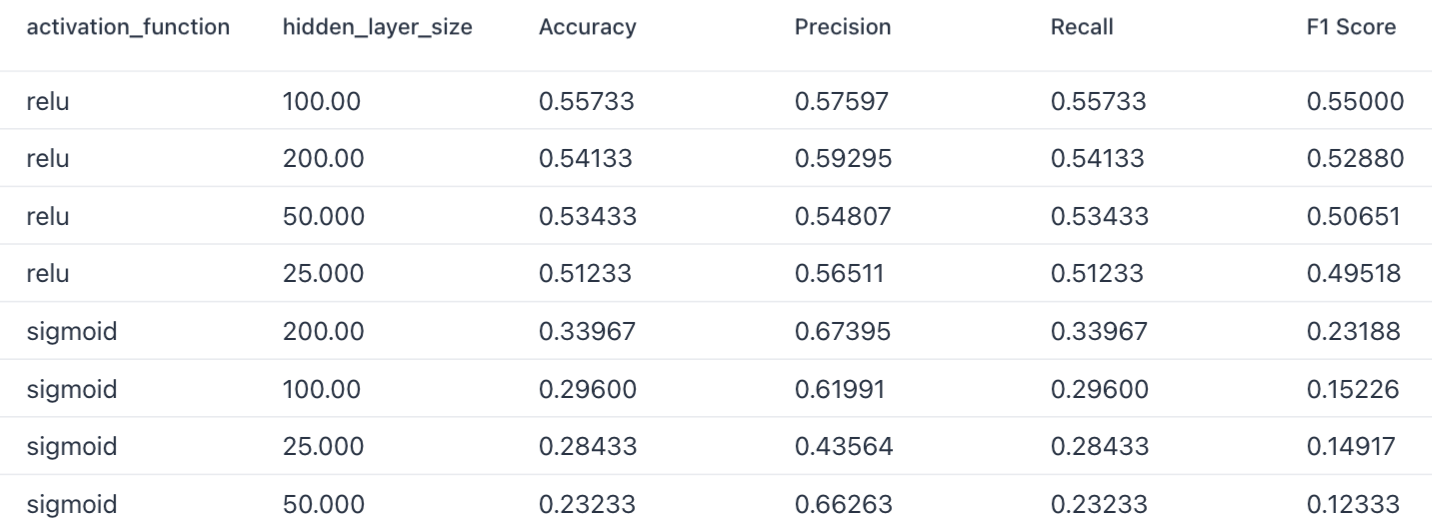
\includegraphics[width=1\linewidth]{images/FNN_tensorboard_table.png}
    \caption{Table containing the hyperparameters and the results of the hypertuning process performed.}
    \label{fig:FNN_table}
\end{figure}
The first model present in the image stands out as the best combination of tuned hyperparameters as it has the best results regarding the performance metrics. This model uses 100 neurons for each hidden layer, and a relu activation function in the three hidden layers. 

The best performance for relu is achieved with a hidden layer size of 100, with the following metrics:
\begin{itemize}
    \item Accuracy: 0.55733
    \item Precision: 0.57597
    \item Recall: 0.55733
    \item F1 Score: 0.55000
\end{itemize}

Sigmoid’s best performance is with a hidden layer size of 200, but its metrics are significantly lower:
\begin{itemize}
    \item Accuracy: 0.33967
    \item Precision: 0.67395
    \item Recall: 0.33967
    \item F1 Score: 0.23188
\end{itemize}

The relu activation function consistently outperforms sigmoid, even the best sigmoid model performs worse than any relu model. This is likely due to its ability to prevent vanishing gradient issues compared to sigmoid. When calculating the gradient for sigmoid its derivative is at most 0.25. The down side of this is when you have many layers the multiplication of these gradients tend to zero very quickly \cite{vanishing_grad}. 

The next figure provides a visual representation of the accuracy and loss trends for both training and validation data across the hyperparameter model over \textbf{30 epochs}, offering insights into the model's learning dynamics.

\begin{figure}[H]
    \centering
    \begin{subfigure}[t]{0.35\textwidth} % Tamanho de cada subfigura
        \centering
        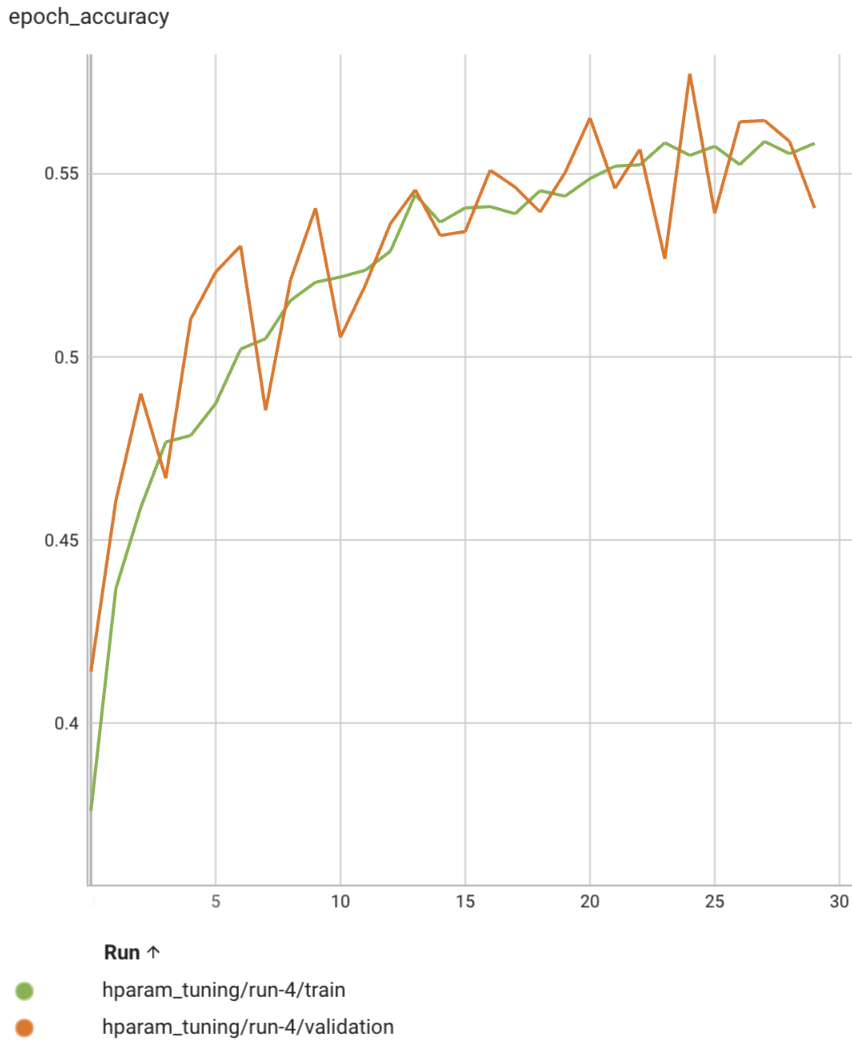
\includegraphics[width=\textwidth]{images/fnn_epoch_accuracy.png}
        \caption{Train vs Validation Accuracy over epochs}
        \label{fig:fnn_subfig1}
    \end{subfigure}
    \hfill
    \begin{subfigure}[t]{0.30\textwidth}
        \centering
        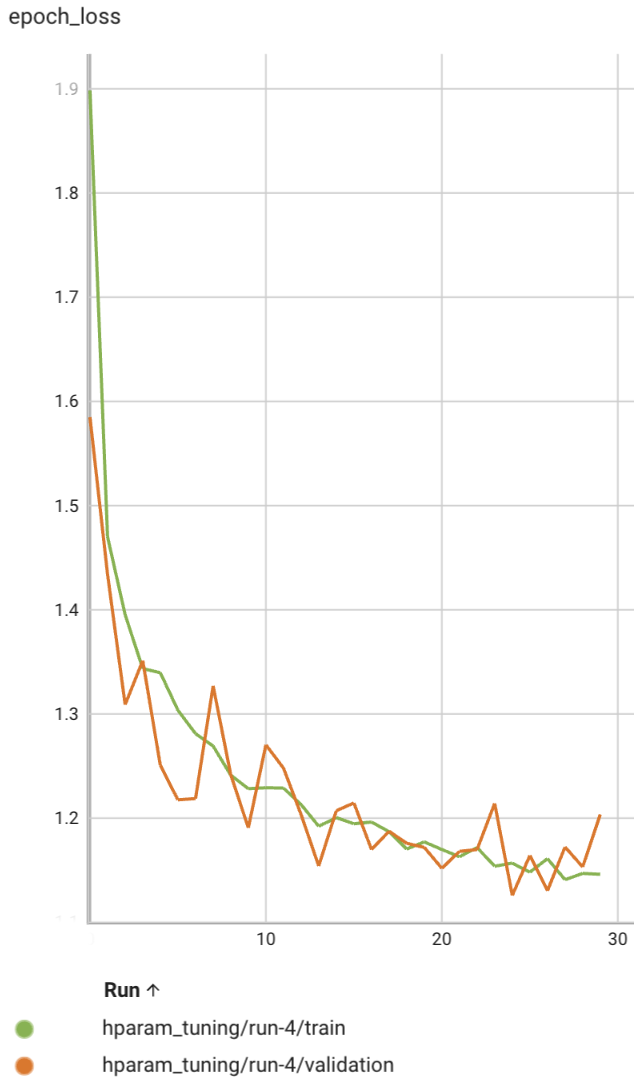
\includegraphics[width=\textwidth]{images/fnn_epoch_loss.png}
        \caption{Train vs Validation Loss over epochs}
        \label{fig:fnn_subfig2}
    \end{subfigure}
    \caption{Accuracy and Loss over epoch for the best set of hyperparameters FNN model.}
    \label{fig:images}
\end{figure}

As we can see in the first chart the training stabilizes by the 20th epoch, indicating that further training brings no significant improvements. The validation accuracy follows a similar trend to the training accuracy, increasing steadily during the early epochs. However, it also stabilizes after the 20th epoch. Both training and validation accuracies converge near the end of training. This suggests the model's performance on the validation set is close to that on the training set, suggesting good generalization. We can see there is little to no gap in both images between the training and validation curves which indicates the model does not overfit the training data.

To gain a deeper understanding of the model's performance, we can analyze the generated confusion matrix for the test data in the following image.
\begin{figure}[H]
    \centering
    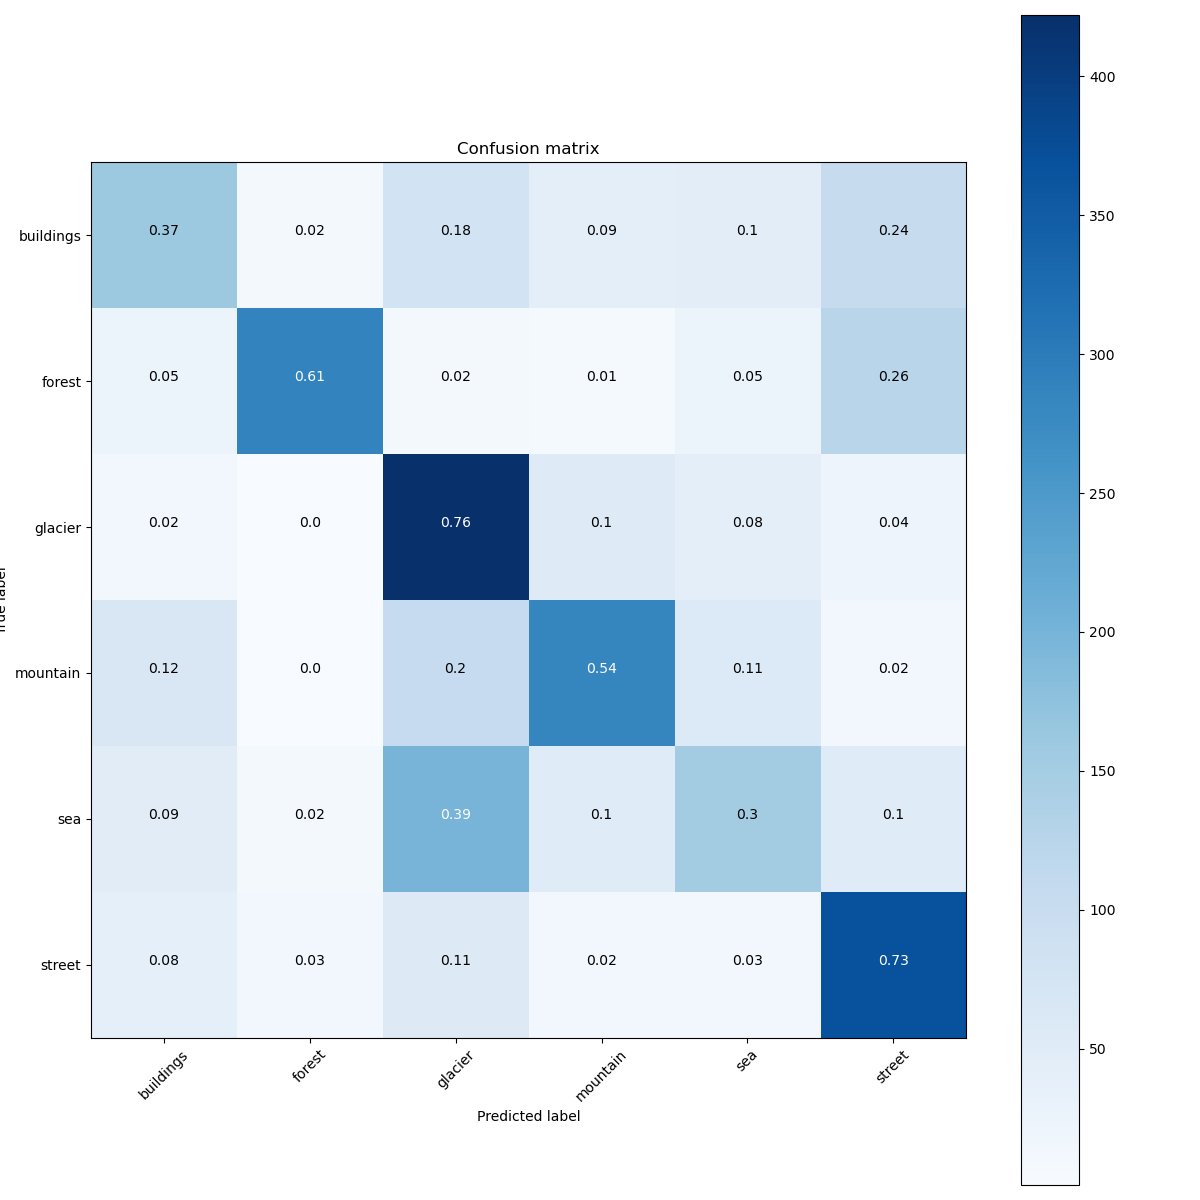
\includegraphics[width=1\linewidth]{images/fnn_cm.png}
    \caption{Confusion matrix of the best hyperparameter FNN model.}
    \label{fig:FNN_cm}
\end{figure}
This confusion matrix indicates the classes with the highest correct prediction rates are glacier and street, and the more challenging classes are buildings and sea. 

\subsection{Convolutional Neural Networks (CNNs)}
This CNNs approach uses a Data Augmentation training and validation set which is similar to the one used in the FNN approach described before.

The model architecture includes three convolutional layers, each followed by a max-pooling layer, with a fully connected dense layer and a dropout layer for regularization before the output layer. It is structured in the following table.

\begin{table}[H]
\centering
\caption{Architecture of the CNN Model}
\begin{tabular}{|l|}
\hline
\textbf{Layer (Type)}\\ \hline
Conv2D                      \\ \hline
MaxPooling2D                \\ \hline
Conv2D                      \\ \hline
MaxPooling2D                \\ \hline
Conv2D                      \\ \hline
MaxPooling2D                \\ \hline
Flatten                     \\ \hline
Dense                       \\ \hline
Dropout                     \\ \hline
Dense                  \\
\hline
\end{tabular}
\label{tab:cnn_architecture_2}
\end{table}

A grid search approach of hypertuning the model was used. It consisted of trying out different values of the hyperparameters and picking the "model" that gives the best score. This approach was used for balancing computational efficiency and thoroughness in exploring hyperparameter combinations. The hyperparameters that were tuned are the kernel/filter size, the dropout rate, and the optimizer function. The values experimented of each hyperparameter can be consulted in the table \ref{tab:cnn_hypertuning}.

\begin{table}[H]
\centering
\caption{CNN tuned hyperparameters.}
\begin{tabular}{|l|c|}
\hline
\textbf{Hyperparameter} & \textbf{Values} \\ \hline
Filter size & \{3, 5, 7\} \\ \hline
Dropout rate & \{0.2, 0.5\} \\ \hline
Otimizer & \{adam, sgd\} \\ \hline
\end{tabular}
\label{tab:cnn_hypertuning}
\end{table}

For each model created with a different set of hyperparameters the test confusion matrix and performance metrics were registered. This registration was made with the help of TensorBoard. Tensorboard is a python package that provides "visualization and tooling needed for machine learning experimentation"\cite{tensorboard}. It was instrumental in monitoring training and validation loss curves, ensuring proper convergence. The results for each model are kept in a logs folder which facilitates its detailed analysis.

In the image \ref{fig:CNN_table} all the performance metrics evaluated along with the tuned hyperparameters are exhibited.
\begin{figure}[H]
    \centering
    \includegraphics[width=1\linewidth]{images/CNN_tensorboard_table.png}
    \caption{Table containing the hyperparameters and the results of the hypertuning performed.}
    \label{fig:CNN_table}
\end{figure}
The first model present in the image stands out as the best combination of tuned hyperparameters as it has the best results regarding the performance metrics. It uses the adam optimizer, a kernel size of 3, and a dropout rate of 0.5. From the results we can understand that Adam consistently outperforms SGD. Smaller kernel sizes (3 or 5) generally perform better, with Adam paired with kernel size of 3 being the most effective.

The next figure provides a visual representation of the accuracy and loss trends for both training and validation data across the hyperparameter model over \textbf{30 epochs}, offering insights into the model's learning dynamics.

\begin{figure}[H]
    \centering
    \begin{subfigure}[t]{0.35\textwidth} % Tamanho de cada subfigura
        \centering
        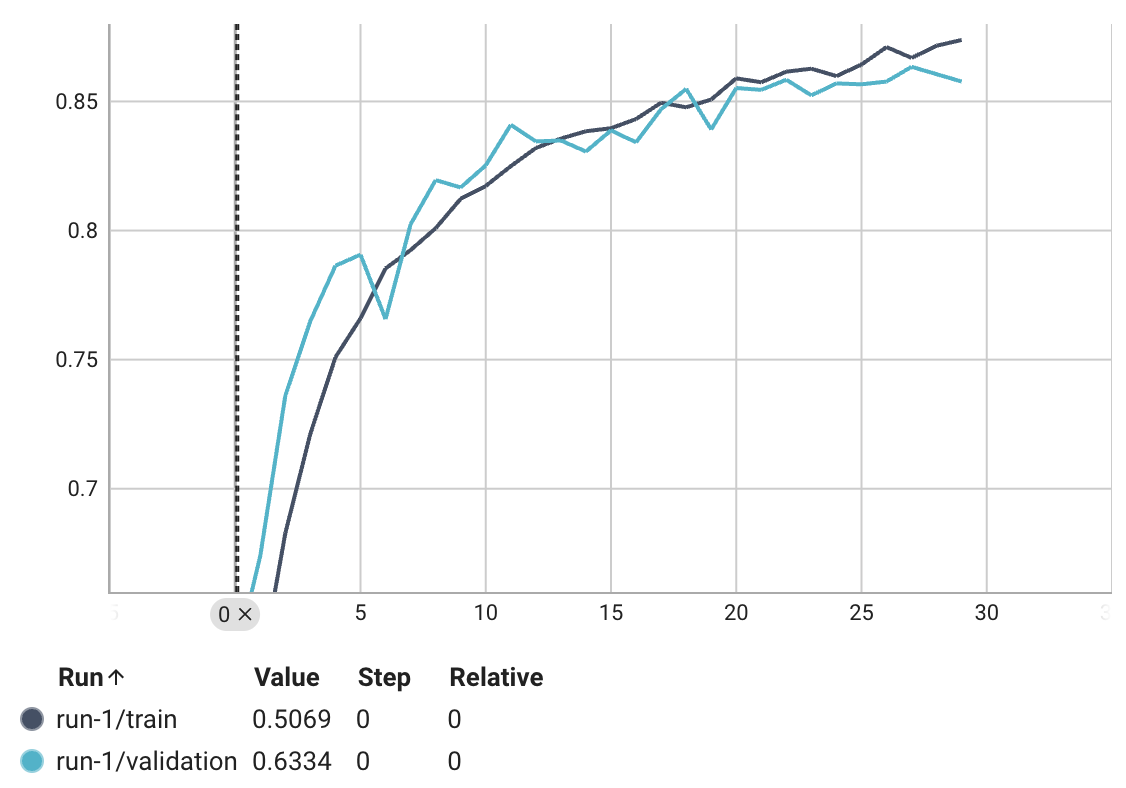
\includegraphics[width=\textwidth]{images/cnn_epoch_accuracy.png}
        \caption{Train vs Validation Accuracy over epochs}
        \label{fig:cnn_subfig1}
    \end{subfigure}
    \hfill
    \begin{subfigure}[t]{0.30\textwidth}
        \centering
        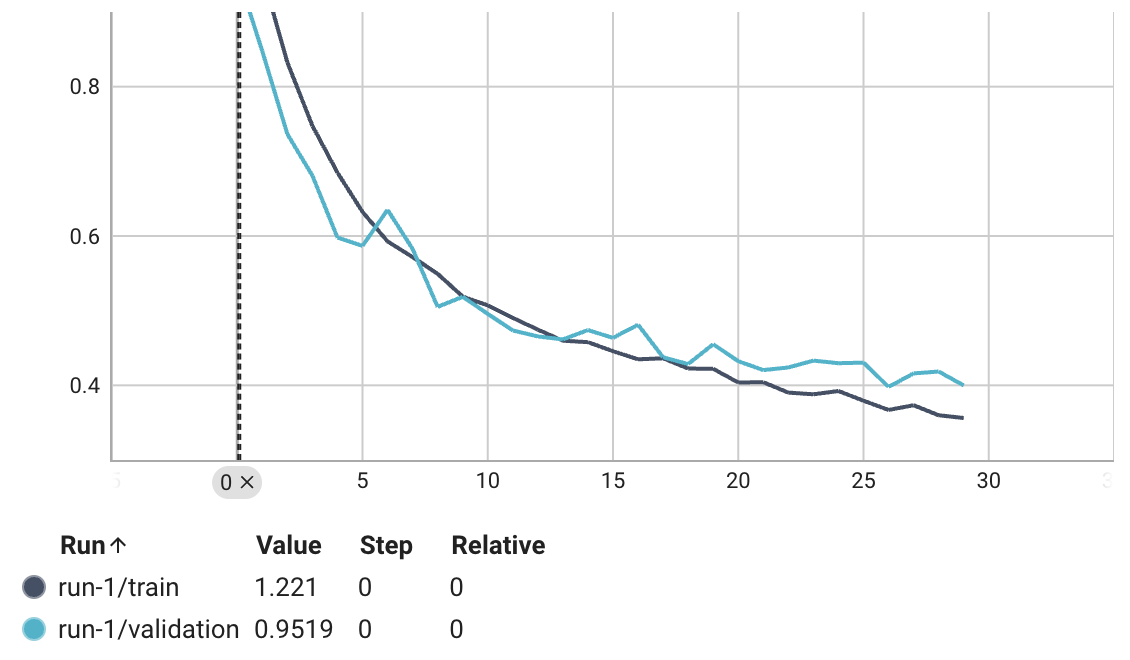
\includegraphics[width=\textwidth]{images/cnn_epoch_loss.png}
        \caption{Train vs Validation Loss over epochs}
        \label{fig:cnn_subfig2}
    \end{subfigure}
    \caption{Accuracy and Loss over epoch for the best set of hyperparameters CNN model.}
    \label{fig:images}
\end{figure}

As we can see in the first chart the training stabilizes by the 20th epoch, indicating that further training brings no significant improvements. The validation accuracy follows a similar trend to the training accuracy, increasing steadily during the early epochs. However, it also stabilizes after the 20th epoch. Both training and validation accuracies converge near the end of training. This suggests the model's performance on the validation set is close to that on the training set, suggesting good generalization. We can see there is little to no gap in both images between the training and validation curves which indicates the model does not overfit the training data.

To gain a deeper understanding of the model's performance, we can analyze the generated confusion matrix for the test data in the following image.
\begin{figure}[H]
    \centering
    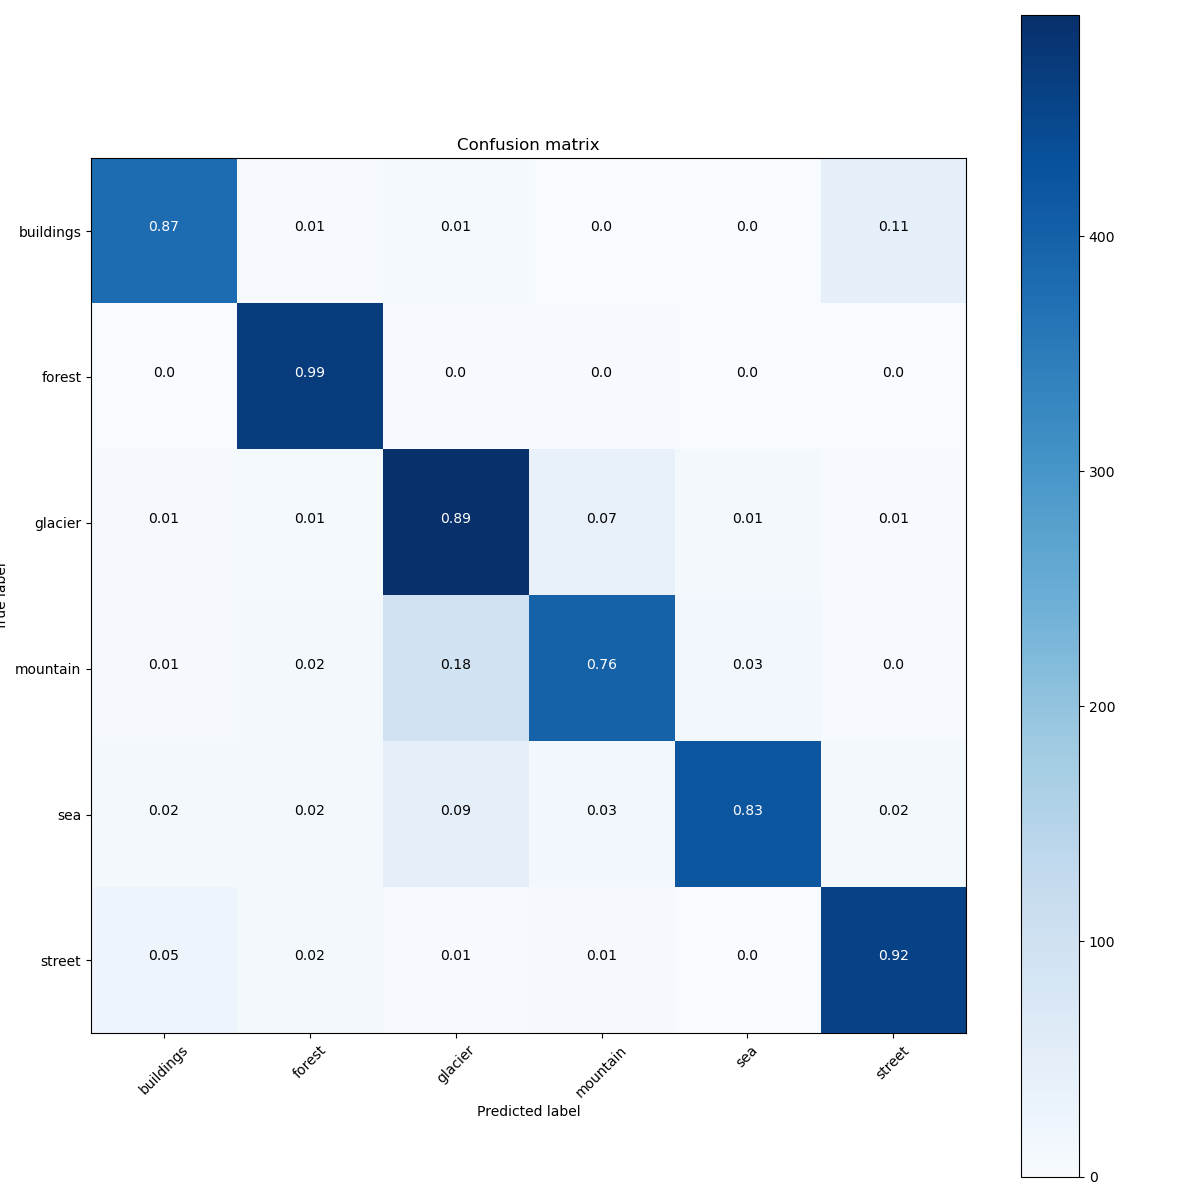
\includegraphics[width=1\linewidth]{images/cnn_tensorboard_cm.png}
    \caption{Confusion matrix of the best hyperparameter CNN model.}
    \label{fig:CNN_cm}
\end{figure}

The confusion matrix indicates the model performs exceptionally well on Forest and Street classes, suggesting strong feature extraction and learning for these categories. Overall there is minimal missclassifications which highlights the robustness of the model in distinguishing between classes.
The largest source of misclassification are mountains vs glaciers, 18\% of mountains are predicted as glaciers. This suggests overlapping features or insufficiently distinct feature extraction for these classes. The 11\% missclassification rate for buildings as streets show that urban environments are challenging to classify.

\subsection{DenseNet Model}

This model utilizes the DenseNet121 architecture, which is a deep convolutional network designed to improve feature reuse through dense connections. Instead of using simple convolutional layers, DenseNet121 employs a more complex design with dense blocks, where each layer receives input from all previous layers, allowing the model to learn more complex representations while reducing the number of parameters.

In this implementation, the pre-trained weights from ImageNet are used for feature extraction. The DenseNet121 model is fine-tuned by adding a Global Average Pooling layer followed by a fully connected dense layer with 128 units and a ReLU activation. To prevent overfitting, a Dropout layer with a rate of 0.5 is applied before the final output layer. The output layer consists of 6 units with a Softmax activation, designed to classify the images into one of six categories.

The model was compiled using the Adam optimizer with a default learning rate of 0.001. The Adam optimizer is well suited for this task due to its adaptive learning rate capabilities.
The loss function used is ”categorical crossentropy”, which is appropriate for multiclass classification problems, and the performance metric tracked during training was accuracy.
The performance of the DenseNet model was evaluated using training, validation, and test datasets. The model demonstrated a high accuracy on the training data but showed a significant drop in accuracy on the validation and test data, indicating potential overfitting.

The next figure provides a visual representation of the accuracy and loss trends for both training and validation data across the \textbf{30 epochs}, offering insights into the model's learning dynamics.
The model achieved higher accuracy on the training data compared to the validation and test data. This discrepancy suggests potential overfitting, where the model performs well on the data it has seen but struggles to generalize effectively to unseen data.
This behavior is further corroborated by the loss values recorded during training and validation, which highlight the challenges in maintaining consistency across datasets.

\begin{figure}[H]
    \centering
    \begin{subfigure}[t]{0.45\textwidth} 
        \centering
        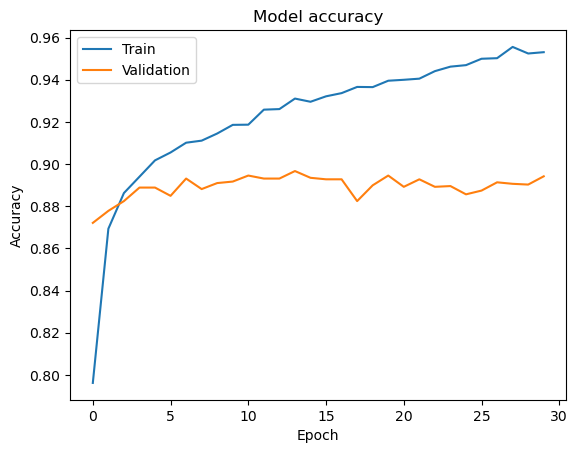
\includegraphics[width=\textwidth]{images/densenet_accuracy.png}
        \caption{Train vs Validation Accuracy}
        \label{fig:subfig1}
    \end{subfigure}
    \hfill
    \begin{subfigure}[t]{0.45\textwidth}
        \centering
        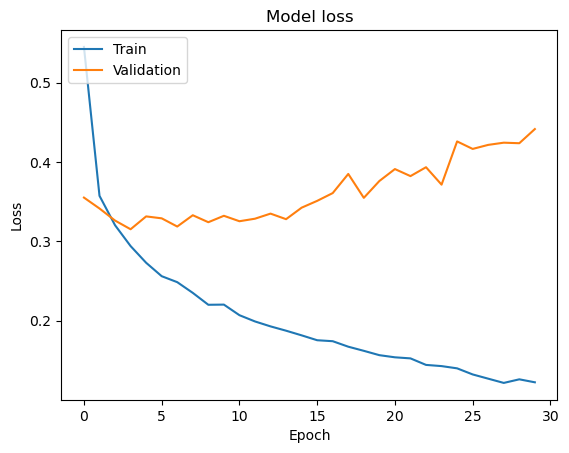
\includegraphics[width=\textwidth]{images/densenet_loss.png}
        \caption{Train vs Validation Loss}
        \label{fig:subfig2}
    \end{subfigure}
    \caption{Accuracy and Loss for the DenseNet Model}
    \label{fig:images}
\end{figure}

The graphs reveal that while the training accuracy consistently improves and the training loss decreases, the validation accuracy stagnates after the initial epochs, and the validation loss increases. This pattern further reinforces the indication of overfitting.

To gain a deeper understanding of the model's performance, we generated the confusion matrix for the test data and calculated the precision, recall, and F1-score, providing a more comprehensive evaluation of the model's effectiveness across different classes.


\begin{figure}[H]
    \centering
    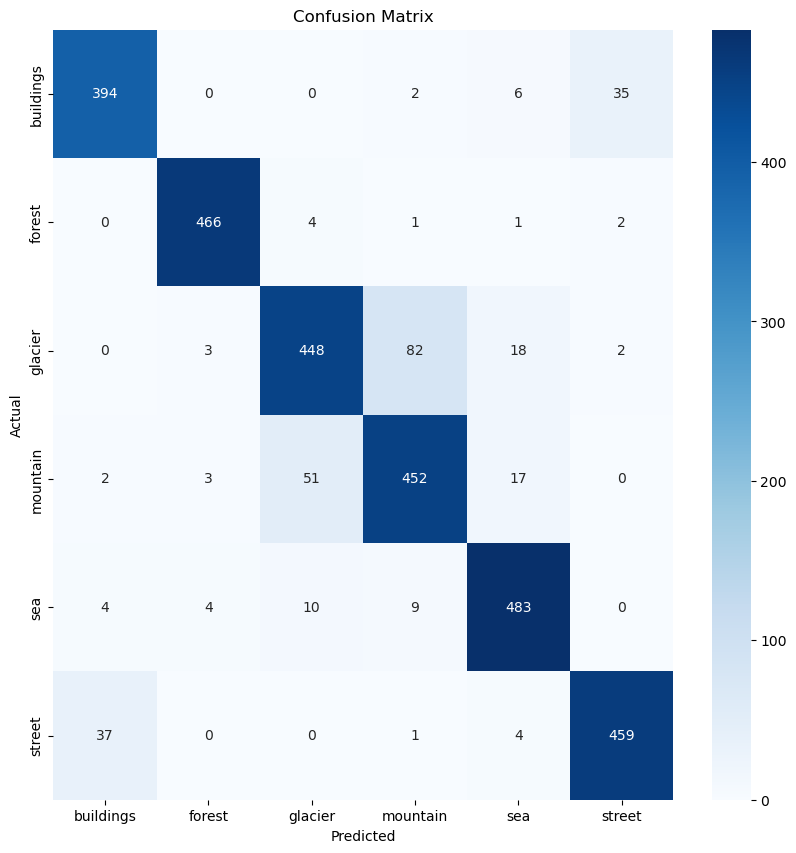
\includegraphics[width=1\linewidth]{images/densenet_confusion.png}
    \caption{Model Confusion Matrix}
    \label{fig:enter-label}
\end{figure}

\begin{figure}[H]
    \centering
    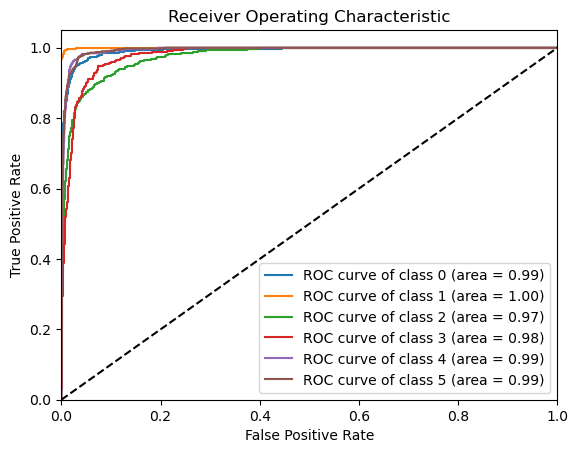
\includegraphics[width=1\linewidth]{images/densenet_roc.png}
    \caption{Roc Curve}
    \label{fig:rocincial}
\end{figure}

\begin{table}[H]
    \centering
    \caption{Model Test Evaluation Metrics} 
    \begin{tabular}{||c|c|c|c|c||} 
        \hline
        Accuracy & F1 Score & Recall & Precision \\
        \hline\hline
        0.900 & 0.900 & 0.901 & 0.901 \\
        \hline
    \end{tabular}
    \label{tab:tab_LogReg}
\end{table}

Forests (1) are classified very accurately, with the majority of predictions falling into the correct category. Buildings (0), however, are still often misclassified as Streets (5), with 35 misclassifications, and Streets (5) are sometimes confused with Buildings (0). Despite these challenges, the model shows significant improvements in overall performance. However, there remains a notable overlap between certain classes. Mountains (3) and Glaciers (2) are still frequently confused with each other, reflecting their visual similarities, with 82 mountains misclassified as glaciers and 51 glaciers misclassified as mountains. Similarly, there is still confusion between Streets (5) and Buildings (0), highlighting the difficulty in distinguishing these two categories due to their structural similarities in the dataset.

The ROC (Receiver Operating Characteristic) curves for the six scene classes provide an overall view of the model’s ability to distinguish between different types of scenery. Each ROC curve plots the true positive rate against the false positive rate, with the Area Under the Curve (AUC) representing the
model’s performance. As it can be seen in the ROC curve, all classes, except for Glaciers (2), performed very closely to achieving perfect results, with only minor deviations. Class 1 (Forest) achieved the best AUC value, showing the highest accuracy in distinguishing its category. However, Glaciers (2) fell short in comparison to the other categories, with a significantly lower AUC score, indicating more difficulty in distinguishing this class from the others.


\subsection{DenseNet with Data Augmentation}

This model follows the same architecture as the previous model, but with the addition of data augmentation to enhance the model's ability to generalize. Data augmentation techniques, including random rotations, width and height shifts, zooming, shearing, and horizontal flipping, were applied to the training data. These transformations aim to create a more diverse set of images for training, which helps in reducing overfitting.


\begin{figure}[H]
    \centering
    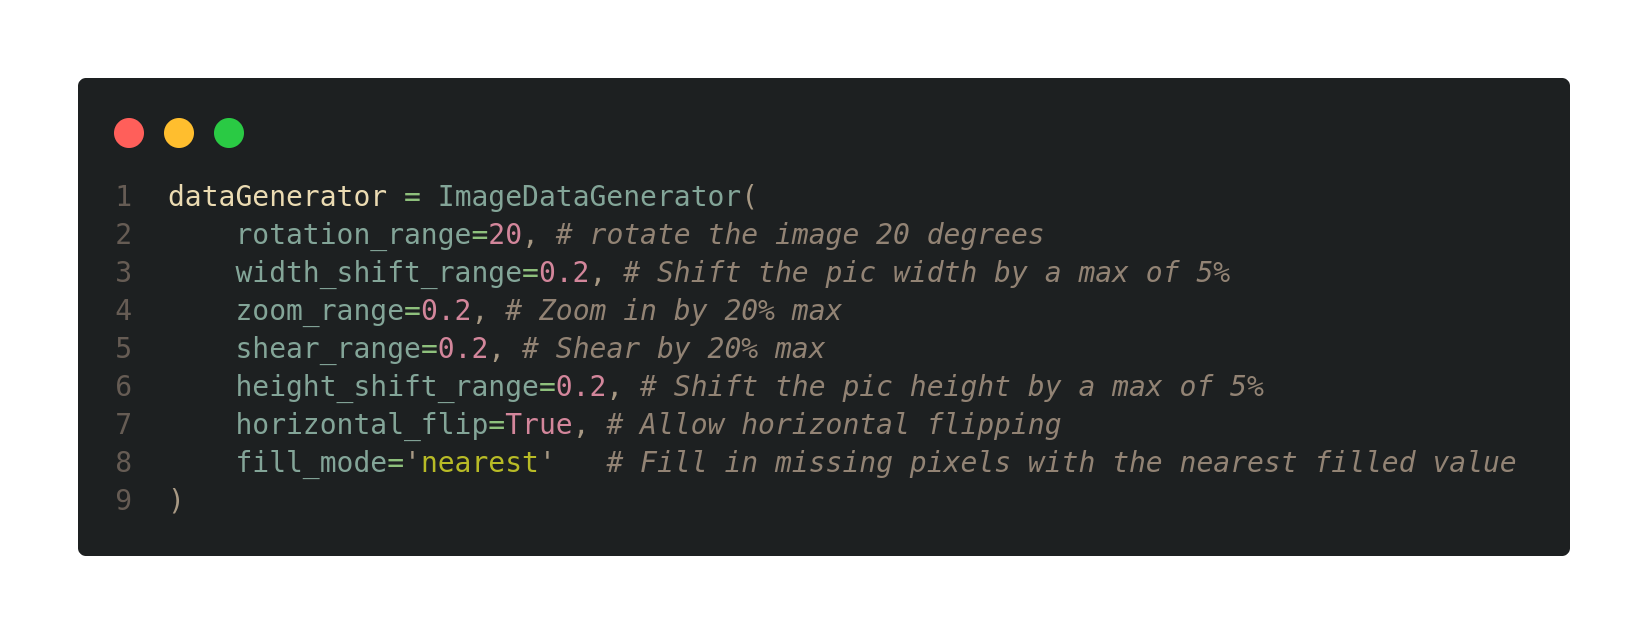
\includegraphics[width=1\linewidth]{images/modelo_aulas_dataaug.png}
    \caption{Data Augmentation Applied}
    \label{fig:enter-label}
\end{figure}

The next figure provides a visual representation of the accuracy and loss trends for both training and validation data across the \textbf{30 epochs}, offering insights into the model's learning dynamics.


\begin{figure}[H]
    \centering
    \begin{subfigure}[t]{0.45\textwidth} 
        \centering
        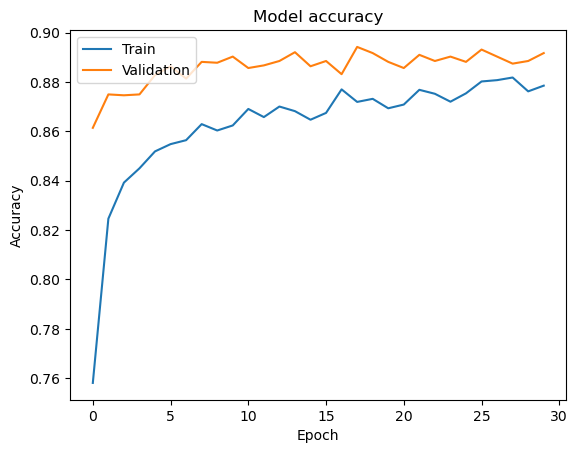
\includegraphics[width=\textwidth]{images/densenet_accuracy_dataaug.png}
        \caption{Train vs Validation Accuracy}
        \label{fig:subfig1}
    \end{subfigure}
    \hfill
    \begin{subfigure}[t]{0.45\textwidth}
        \centering
        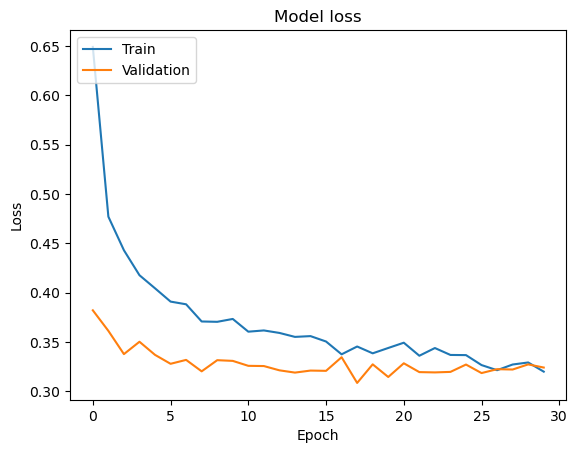
\includegraphics[width=\textwidth]{images/densenet_loss_dataaug.png}
        \caption{Train vs Validation Loss}
        \label{fig:subfig2}
    \end{subfigure}
    \caption{Accuracy and Loss for the DenseNet Model with Data Augmentation}
    \label{fig:images}
\end{figure}

The graphs reveal that, unlike the model without data augmentation, the discrepancy between training and validation performance is no longer evident. The training accuracy consistently improves while the validation accuracy closely follows, remaining slightly higher throughout the epochs. Additionally, the training and validation loss curves align more closely, indicating that the model benefits from the data augmentation, reducing overfitting and generalizing better to unseen data.

To gain a deeper understanding of the model's performance, we generated the confusion matrix for the test data and calculated the precision, recall, and F1-score, providing a more comprehensive evaluation of the model's effectiveness across different classes.


\begin{figure}[H]
    \centering
    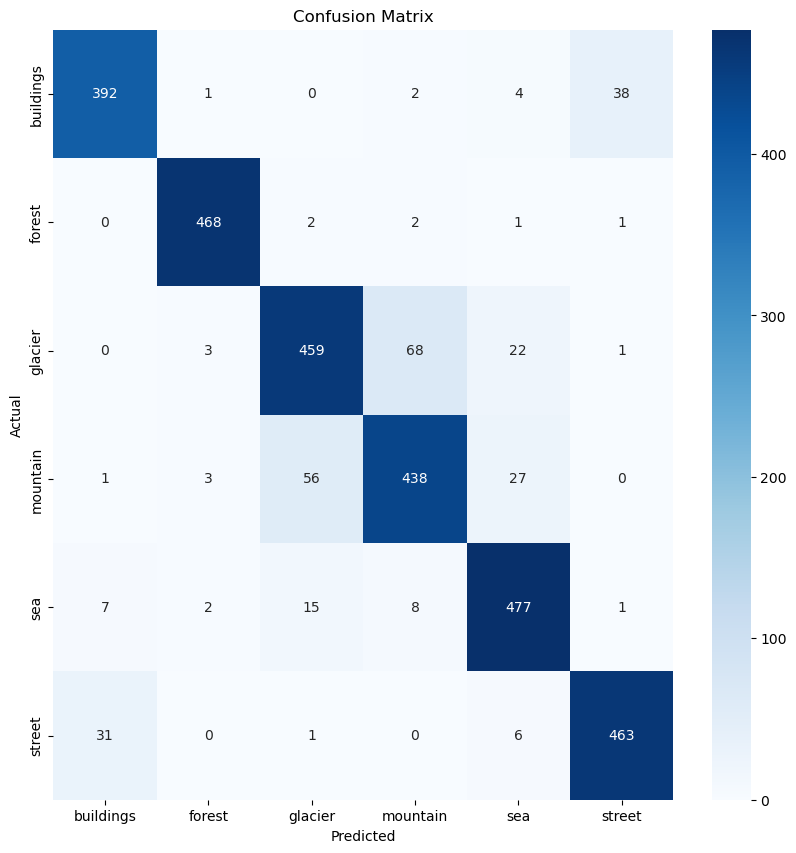
\includegraphics[width=1\linewidth]{images/densenet_confusion_dataug.png}
    \caption{Model Confusion Matrix}
    \label{fig:enter-label}
\end{figure}
\begin{figure}[H]
    \centering
    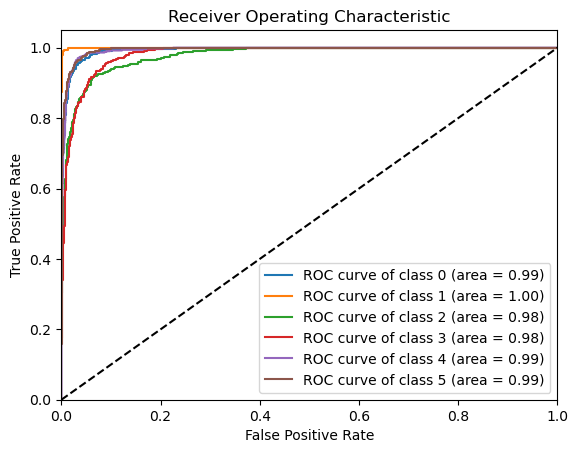
\includegraphics[width=1\linewidth]{images/densenet_roc_aug.png}
    \caption{Roc Curve}
    \label{fig:rocincial}
\end{figure}

\begin{table}[H]
    \centering
    \caption{Model Test Evaluation Metrics} 
    \begin{tabular}{||c|c|c|c|c||} 
        \hline
        Accuracy & F1 Score & Recall & Precision \\
        \hline\hline
        0.899 & 0.899 & 0.899 & 0.899 \\        
        \hline
    \end{tabular}
    \label{tab:tab_LogReg}
\end{table}



With the DenseNet model and data augmentation applied, Forests (1) remain the best-classified category, with the majority of predictions falling correctly into this class. Additionally, Sea (4) also demonstrates strong performance, showing considerable improvement.

However, the model still struggles to differentiate Buildings (0) and Streets (5), with misclassifications increasing slightly from 35 to 38. The confusion between Glaciers (2) and Mountains (3) persists, though it has improved significantly compared to earlier results. These improvements highlight the potential of DenseNet with data augmentation in addressing some classification challenges while leaving room for further refinement in distinguishing between visually similar categories.

The ROC (Receiver Operating Characteristic) curves for the six scene classes provide an insightful overview of the model’s capacity to differentiate between various types of scenery. Each curve represents the true positive rate against the false positive rate, with the Area Under the Curve (AUC) reflecting overall performance.

With the DenseNet model and data augmentation applied, results remain largely consistent, with notable improvements across some classes. For instance, Glaciers (2), previously a weaker category, now exhibits a much stronger AUC score, with values ranging between 0.98 and 1, demonstrating a significant enhancement in distinguishing this class. Other classes, including Forests (1), continue to show near-perfect performance, maintaining AUC values very close to 1. These results underline the model’s progress in achieving robust classification across most categories.



























\subsection{Comparison between the models}

The comparison between the models is based on the following performance metrics: Accuracy, F1 Score, Recall, and Precision. These metrics allow us to assess how well the models perform in terms of both correctly classifying positive and negative cases and minimizing false positives and false negatives.

\begin{itemize}
    \item \textbf{Accuracy} measures the overall correctness of the model by calculating the ratio of correct predictions to the total number of predictions.
    \item \textbf{F1 Score} is the harmonic mean of Precision and Recall, providing a balance between the two, especially when dealing with imbalanced classes.
    \item \textbf{Recall} (or True Positive Rate) measures the ability of the model to correctly identify positive instances.
    \item \textbf{Precision} measures the accuracy of positive predictions made by the model.
\end{itemize}

\begin{table}[ht]
    \centering
    \caption{Comparison of Models} 
    \begin{tabular}{||c|c|c|c|c||} 
     \hline    
     \textbf{Model} & \textbf{Accuracy} & \textbf{F1 Score} & \textbf{Recall} & \textbf{Precision} \\
     \hline \hline
     CM & 0.834 & 0.834 & 0.834 & 0.835 \\
     \hline
     CM - DA & 0.823 & 0.828 & 0.829 & 0.832 \\
     \hline
          FNN - ReLU & 0.557 & 0.550 & 0.557 & 0.578 \\
     \hline
    CNN - Hyper & 0.875 & 0.875 & 0.875 & 0.879 \\
    \hline
     DN & 0.900 & 0.900 & 0.901 & 0.901 \\
     \hline 
     DN - DA & 0.899 & 0.899 & 0.899 & 0.899 \\
     \hline
\hline
     \multicolumn{5}{||c||}{\textbf{Models Name}} \\
     \hline
     CM & \multicolumn{4}{|l||}{CNN Class Model} \\ 
     \hline
     CM - DA & \multicolumn{4}{|l||}{CNN Class Model with Data Augmentation} \\ 
     \hline
          FNN - ReLU & \multicolumn{4}{|l||}{FNN ReLU Activation Function (Hidden Layer Size 100)} \\ 
     \hline
         CNN - Hyper & \multicolumn{4}{|l||}{Best Hyper Tunned CNN} \\ 
    \hline
     DN & \multicolumn{4}{|l||}{DenseNet Model} \\ 
     \hline
     DN - DA & \multicolumn{4}{|l||}{DenseNet Model with Data Augmentation} \\ 
     \hline

    \end{tabular}
    \label{tab:tab_Final_results}
\end{table}


Based on the results in Table \ref{tab:tab_Final_results}, we can observe the following:

The DenseNet model (DN) achieved the highest accuracy (90.0) among all models tested, indicating its superior ability to capture and utilize complex features within the Intel Image Classification dataset. The model's performance remained robust even with the application of data augmentation (DN - DA), showing a marginal reduction in accuracy to 89.9. This highlights DenseNet's resilience and strong generalization capabilities.

The CNN Class Model (CM) exhibited a respectable accuracy of 83.4, demonstrating the effectiveness of convolutional layers for feature extraction in image classification tasks. However, when data augmentation was applied (CM - DA), the model's accuracy slightly decreased to 82.3. This indicates that while data augmentation can enhance variability in the training set, it may not always lead to improved performance, particularly in simpler CNN architectures.

The hyperparameter-tuned CNN (CNN - Hyper) performed significantly better than the base CNN model, achieving an accuracy of 87.5. This underscores the importance of hyperparameter optimization in achieving better results without requiring the deeper architectures of DenseNet.

The FNN model yielded poor results, with an accuracy of 55.7. This highlights the limitations of fully connected architectures in handling image data, as they lack the spatial feature extraction capabilities inherent in CNNs and DenseNet.

The impact of data augmentation varied between models. For DenseNet, the performance with data augmentation (DN - DA) was almost identical to the version without it, suggesting that the model already effectively generalized across the dataset. However, for the simpler CNN model (CM - DA), data augmentation led to a slight performance decline.
\section{Comparison with State-of-the-Art Methods}

To evaluate the performance of our models in the context of state-of-the-art solutions, we compared our results to several notable studies and Kaggle notebooks that utilized the Intel Image Classification dataset. These works employ a diverse range of techniques, from traditional machine learning to advanced deep learning models, allowing us to position our findings within the current research landscape.

\begin{enumerate}
    \item Image Classification Using Modified Convolutional Neural Network: 
In the study \textit{Image Classification Using Modified Convolutional Neural Network} \cite{khan2024image}, the authors employed CNNs to classify images in the Intel Image Classification dataset. Their architecture utilized convolutional layers to extract basic features (e.g., edges and corners), followed by fully connected layers to capture more complex patterns. The model achieved solid performance with a Softmax function for multiclass classification. Additionally, K-Nearest Neighbors (KNN) was employed using a "Bag-Of-Features" approach for feature extraction, with 80 of the top features retained per category. This hybrid approach provides an interesting comparison to our own, particularly in terms of how the models handle feature extraction.
 
    
    \item Kaggle Notebook Using a Custom CNN Architecture: 
In a separate Kaggle notebook \cite{kaggle2024intel}, the author developed a custom CNN with three convolutional layers followed by max pooling and dense layers. This design was simple yet effective, aimed at extracting hierarchical features to classify the six categories in the dataset. The performance of this model offers a baseline against which we can compare our results, especially regarding its ability to capture spatial relationships and distinguish between the classes.


    \item Kaggle Notebook Using DenseNet:
A third Kaggle notebook utilized the DenseNet architecture \cite{kaggle2023densenet}, a more advanced deep learning model known for its efficiency in capturing complex patterns through its dense connectivity between layers. This structure promotes feature reuse and enhances gradient flow, making it well-suited for tasks requiring the extraction of intricate features from images. DenseNet's performance, especially with deep and dense architectures, offers a high bar for comparison, particularly in tasks where feature complexity and high-level abstractions are key to classification accuracy.
\end{enumerate}

After reviewing these state-of-the-art models, we performed a comparison of our results with those obtained from the studies mentioned above. The following tables summarize the performance of our models and those from the literature, focusing on accuracy metric.

\begin{table}[H]
    \centering
    \caption{Our Models Results} 
    \begin{tabular}{||c|c|c|c|c||} 
     \hline    
     \textbf{Model} & \textbf{Accuracy} & \textbf{F1 Score} & \textbf{Recall} & \textbf{Precision} \\
     \hline \hline
     CM & 0.834 & 0.834 & 0.834 & 0.835 \\
     \hline
    CNN - Hyper & 0.875 & 0.875 & 0.875 & 0.879 \\
     \hline
     DN & 0.900 & 0.900 & 0.901 & 0.901 \\
     \hline 

\hline
     \multicolumn{5}{||c||}{\textbf{Models Name}} \\
     \hline
     CM & \multicolumn{4}{|l||}{CNN Class Model} \\ 
     \hline
    CNN - Hyper & \multicolumn{4}{|l||}{Best Hyper Tunned CNN} \\ 
     \hline
     DN & \multicolumn{4}{|l||}{DenseNet Model} \\ 
\hline

    \end{tabular}
    \label{tab:tab_Final}
\end{table}


\begin{table}[H]
    \centering
    \caption{Custom CNN Architecture Kaggle notebook\cite{kaggle2024intel}} 
    \begin{tabular}{||c|c|c|c||} 
     \hline    
     \textbf{Stage} & \textbf{Accuracy} & \textbf{Loss} \\
     \hline \hline
     Training (Step 1) & 0.9453 & 0.1933  \\
     \hline
     Training (Step 2) & 0.9186 & 0.2581 \\
     \hline
     Testing & 0.8314 & 0.4845 \\
     \hline
    \end{tabular}
    \label{tab:model_evaluation}
\end{table}

\begin{table}[H]
    \centering
    \caption{DenseNet Kaggle notebook\cite{kaggle2023densenet}}
    \begin{tabular}{||c|c|c|c||} 
     \hline    
     \textbf{Stage} & \textbf{Accuracy} & \textbf{Loss} \\
     \hline \hline
     Training  & 0.9117 & 0.2459  \\
     \hline
     Validation & 0.8820 & 0.3308\\
     \hline
     Testing & 0.8887 & 0.3084  \\

     \hline
    \end{tabular}
    \label{tab:model_evaluation_epoch17}
\end{table}


\begin{table}[H]
    \centering
    \caption{\textit{Image Classification Using Modified Convolutional Neural Network} \cite{khan2024image}} 
    \begin{tabular}{||c|c|c|c|c||} 
     \hline    
     \textbf{Method} & \textbf{KNN} & \textbf{Best CNN}  \\
     \hline \hline
     \textbf{Accuracy} & 85.3704 & 93.61 \\
     \hline
    \end{tabular}
    \label{tab:classification_comparison}
\end{table}



\textbf{Our Models Results (Table \ref{tab:tab_Final}):}
\begin{itemize}
    \item CNN Class Model (CM): Achieved an accuracy of 83.4, with balanced F1 score, recall, and precision metrics, making it a competitive baseline.
    \item Hyper-Tuned CNN (CNN-Hyper): Improved upon the CM by achieving an accuracy of 87.5, reflecting the benefits of hyperparameter tuning in optimizing the CNN's architecture.
    \item DenseNet (DN): Demonstrated the highest performance among our models, with 90 accuracy and similarly high F1 score, recall, and precision. DenseNet's dense connectivity allows for better gradient flow and feature reuse, making it superior in handling complex image datasets.
\end{itemize}

\textbf{Custom CNN Architecture Kaggle Notebook (Table \ref{tab:model_evaluation}):}
\begin{itemize}
    \item The custom CNN architecture achieved a testing accuracy of 83.14, slightly below our hyper-tuned CNN and DenseNet models. While the training accuracy was very high (94.53), the significant drop during testing indicates overfitting.
\end{itemize}

\textbf{DenseNet Kaggle Notebook (Table \ref{tab:model_evaluation_epoch17}):}
\begin{itemize}
    \item The DenseNet implementation achieved a testing accuracy of 88.87, closely aligning with the performance of our DenseNet model. Its robust performance during training (91.17) and validation (88.2) stages highlights DenseNet's generalization capabilities.
\end{itemize}
    
\textbf{Image Classification Using Modified CNN (Table \ref{tab:classification_comparison}):}
\begin{itemize}
    \item The study reported 85.37 accuracy using KNN and 93.61 accuracy with their best CNN implementation. Their CNN model outperformed our DenseNet implementation by a small margin, likely due to architectural optimizations or additional dataset augmentations.
\end{itemize}


Among our models, DenseNet achieved the highest accuracy (90), outperforming both the CNN Class Model (83.4) and the hyperparameter-tuned CNN (87.5). This demonstrates that deeper architectures with enhanced connectivity are more effective at extracting complex features from the Intel Image Classification dataset. The DenseNet implementation from the Kaggle notebook also showed strong performance, with a testing accuracy of 88.87, though it fell slightly short of our DenseNet model. This reinforces DenseNet's capability as a robust architecture for image classification tasks.

Our hyperparameter-tuned CNN struck a balance between simplicity and performance, achieving 87.5 accuracy without the computational complexity of DenseNet, making it suitable for resource-constrained scenarios. However, the custom CNN architecture from the Kaggle notebook, despite achieving high training accuracy (94.53), exhibited a significant drop in testing accuracy (83.14), suggesting overfitting and highlighting the challenges simpler architectures face in generalizing on more complex datasets.

Both our DenseNet model and the DenseNet implementation from the Kaggle notebook consistently outperformed traditional CNN architectures and KNN-based methods, emphasizing DenseNet’s strength in leveraging dense connectivity for feature reuse and improved gradient flow. This superiority was further evidenced in the study \textit{Image Classification Using Modified Convolutional Neural Network}, where KNN achieved 85.37 accuracy, competitive with simpler CNNs but significantly lower than DenseNet. Their best CNN implementation reached 93.61 accuracy, underscoring the importance of carefully designed CNN architectures for achieving state-of-the-art results.

In summary, our DenseNet implementation demonstrated robust generalization and closely aligned with state-of-the-art approaches, validating its effectiveness. The hyper-tuned CNN, while simpler, offers a practical alternative for scenarios with limited resources, achieving competitive performance without the complexity of DenseNet.
\input{3-conclusão}
% printing acronyms
\printglossary[type=\acronymtype,title=Acronyms]

% references section
\bibliography{refs}
\bibliographystyle{IEEEtran}



\end{document}